
%%%%%%%%%%%%%%%%%%%%%%%%%%%%%%%%%%%%%%%%
%%%%%%%%%%%%%%%%%%%%%%%%%%%%%%%%%%%%%%%%
%%%%%%%%%%%%%%%%%%%%%%%%%%%%%%%%%%%%%%%%
%%%%%%%%%%%%%%%%%%%%%%%%%%%%%%%%%%%%%%%%
%%%%%%%%%%%%%%%%%%%%%%%%%%%%%%%%%%%%%%%%
\section{Introduction}\label{sec:intro}
% reviewer comment: too long!
 
%%% Diverse applications of exoskeletons, narrowing down to amplification
\IEEEPARstart{\ta A}{\ta{mplification}} \ta{of human strength is---among the many possible applications of exoskeletons---an especially interesting feedback control problem.}\ra{
\IEEEPARstart{E}{xoskeletons} are a broad category of wearable robot\ra{ic}s with many potential applications.}
\ra{Some}\ta{This problem does not appear in exoskeletons that aim to either recover locomotion capability lost to disease \cite{KwaNoordenMisselCraigPrattNeuhaus2009ICRA,AgrawalHaribHereidFinetMasselinPralyAmesSreenathGrizzle2017Access} or offload the strenuous work of rehabilitation therapy from therapists \cite{SugarHeEA2007TNSRE,KimDeshpande2017IJRR}.}
\ta{Nor is it significant in exoskeletons that aid healthy locomotion with timed power boosts \cite{MooneyRouseHerr2014JNRE,ZhangFiersWitteJacksonPoggenseeAtkesonCollins2017Science,SawickiBeckKangYoung2020JNER}.}
\ra{Exosuits (exoskeletons without rigid structures) have also seen some notable success in this area \cite{LeeKimBakerLongKaravasMenardGalianaWalshJNR2018}.}
\ra{This paper focuses on amplification control systems designed to magnify the physical strength of operators as they attempt non-repetitive, unpredictable tasks.}\ta{To amplify human strength is to treat forces of human origin differently from forces of any other origin.}
\ta{And we frame this problem as designing a pair of compliances (or integral-admittances\footnote{\ta{We prefer `compliance' to `integral-admittance' for brevity, but note that this makes `compliance' a transfer function of position per force.}}) for the human-side interface of the robot and the environment-side interface of the robot.
%Amplification control systems are designed to magnify the physical strength of operators as they attempt non-repetitive, unpredictable tasks with unknown payloads.
Amplification control systems are designed to magnify the physical strength of the operator as the operator interacts with an environment \emph{through the robot} while also reducing the weight and inertia the operator feels from the robot itself. This kind of control allows non-repetitive, unpredictable tasks with unknown payloads.
}

%%% Gravity compenstation is not amplification
\ta{Lifting \emph{fixed} payloads is a simpler problem. These loads can be lifted by directly compensating their nominal weight with actuator torque commands (the ``gravity compensation'' strategy).}
\ta{This compensation could be lifting mostly the exoskeleton itself \cite{KazerooniRacineHuangSteger2005ICRA}, or even offloading the operator's own bodyweight \cite{KongMoonJeonTomizuka2010TMech,LvZhuGregg2018CSM,LinLvGregg2019ACC}.}
\ra{\ta{Proper compensation} requires a decent model of the \ta{mass of the} exoskeleton \ta{and payload}\ra{mass}\ra{, h}\ta{.}}%
\ra{A \ra{backdrivable} system }\ta{In an exoskeleton system that can be easily backdriven by the operator, gravity compensation alone is a passable approach for\ra{ the}} \ra{capability platform application}\ta{lifting well-modeled payloads} \cite{Campbell2018Thesis}.
\ta{However, the operator must still accelerate the full inertia, compensate for any model error, and lift any extra payloads themselves.
The inertia burden can be lessened by adding positive acceleration feedback \cite{Kazerooni2005IROS,KongTomizuka2009TMech}, but all three issues can be addressed by adding force-feedback-based amplification.}

\IEEEpubidadjcol%call to add extra space to the second column of the first page to account for the pubid message (which basically consumes space on the first page).




%% Admittance control is not ampilfication
\ta{Admittance control for exoskeletons \cite{YuRosen2013TCyb,FontanaVertechyMarcheschiSalsedoBergamasco2014RAM,JacobsenOlivier2014Patent,LecoursStongeGosselin2012ICRA} uses force sensor feedback at the human interface\footnote{\ta{Measuring human muscular effort, as can also be accomplished via electromyography (muscle measurement)} \cite{KawamotoSankai2005AR,YoungFerris2016TNSRE}.} in order to increase the human-side compliance, reduce sensitivity to the mass model, and lift unknown loads. But the compliance `increase' is relative to the admittance control plant: a position-controlled robot. Since position-controlled robots have very little compliance \cite{YuRosen2013TCyb,GonzalezAsada2019RAL}, the final human-side compliance of an admittance controller is not necessarily an improvement over the torque-controlled gravity compensation strategy. Additionally, the position-controlled plant of the admittance controller will attenuate all external forces acting on the robot. This attenuation typically deprives the operator of force feedback when they interact with the environment.}


%% Amplification requires two force sensors
\ta{In order to allow bidirectional transmission of forces to coexist with amplification of human strength, the exoskeleton must transmit both amplified forces from the user to the environment and attenuated forces from the environment to the user.
This suggests a force sensor configuration that can distinguish the environment from the user.
Directly measuring the robot--environment interface and the robot--human interface with force sensors allowed \cite{KazerooniGuo1993JDSMC,KazerooniMahoney1991ICRA,KazerooniMahoney1991JDSMC} to control \emph{disparate} admittance behaviors for each interface.%
\footnote{\ta{The HARDIMAN I exoskeleton \cite{MakinsonBodineFitck1969Techreport} attempted to do this as well, but with a flawed approach that neglected multi-joint coordination.}}
But the controller from \cite{KazerooniGuo1993JDSMC} was still not designed to improve the human-side compliance relative to the torque-controlled gravity compensation strategy. It still used admittance control and a position-controlled robot.
In this paper, we use force sensing at the human-robot and actuator-robot interfaces, and this serves the dual purposes of distinguishing the human from the environment and allowing torque control at the joints.
The two interface compliances are then shaped with a cascade of amplification feedback on top of torque-controlled actuators.\footnote{More specifically, we use reaction force sensing series elastic actuators with torque control based on disturbance observers \cite{PaineOhSentis2014TMech,Paine2014Dissertation}.}}

\begin{figure}\centering\footnotesize
	\def\svgwidth{\columnwidth}
	\input{new_first_fig.pdf_tex}
	\caption{\ta{Human--exoskeleton--environment interaction illustrating the concept of amplification. Marker A, the Human (inc. the backpack frame), connects to B, the Exoskeleton (the Apptronik Sagittarius), which connects to C, the Environment (an unknown load). The Human--Exoskeleton connection is force/torque sensitive. In D, E, and F a high-level schematic shows a mass-like exoskeleton (Exo) being acted on by forces to result in acceleration. In E and F the acceleration resulting from each force is shown, and D shows the total acceleration---the sum of the accelerations in E and F. Thanks to amplification control, the acceleration resulting from environment-side and human-side forces are \emph{not equal}, and the human can overpower the environment even though the human-side force is smaller in magnitude than the environment-side force.}
	}\label{fig:newfirst}
\end{figure}

%% Problem of non-passivity
\ta{%
Unfortunately, the problem of non-passivity is inherent to feedback control that conceals inertia. This is an issue regardless of how the inertia was concealed---through positive acceleration feedback \cite{Kazerooni2005IROS} or force feedback \cite{BuergerHogan2007TRO}.
Without passivity, we must fall back to robust control in order to certify such behaviors. 
Most importantly, the exoskeleton's human-facing port---its force--position relationship at the human--robot interface---will be in a feedback interconnection with the human's robot-facing port.
Studies of this feedback interconnection \cite{Kazerooni1990TSMC,BuergerHogan2007TRO,BuergerHogan2006IROS,HeThomasPaineSentis2019ACC} and the human in particular \cite{HeHuangThomasSentis2019IROS,HeHuangThomasSentis2020TNSRE} have modeled the human as a mass-spring-damper system with a range of parameter values. The most variable parameter is stiffness, as this depends on muscle contraction \cite{Hogan1984TAC}.
We must demonstrate that no possible human behavior leads to instability---a robust control problem.
Designing a machine to be passive \cite{ColgateHogan1988IJC,Hogan1989ICRA,ColgateBrown1994ICRA,AdamsHannaford1999TRA} can also be seen as a robust control problem: such designs guarantee stability against a very wide range of 'human' behaviors---the set of all passive transfer functions. Our prior work \cite{ThomasCoholichSentis2019AIM,HeThomasPaineSentis2019ACC,HeHuangThomasSentis2019IROS,HeHuangThomasSentis2020TNSRE} has studied this stability problem for a table-mounted elbow exoskeleton.}


%%% STATEMENT OF CONTRIBUTION... Mention tasks so that they can be referred to in the structuring paragraph
\ta{In this paper, we scale up to a 12 degree of freedom (12-DOF) lower-body exoskeleton with 8 active and 4 passive joints. This includes a new multi-joint coordination approach modeled after humanoid robot controllers for torque-controlled joints \cite{SentisParkKhatib2010TRO,KimEA2016TRO} (e.g. the Valkyrie robot at NASA JSC \cite{RadfordEA2015JFR,PaineEA2015JFR}).}
\ra{present}\ta{More specifically, we contribute a comprehensive framework for achieving amplification control in exoskeletons that have torque-controlled joints and force sensing at the human interface. This contribution comprises (a) an optimization-based controller that determines robot joint torques using a prioritized list of `tasks' and a set of constraints that act on the sum of human and robot torques---the `Shared-Body Controller' (Sec.~\ref{sec:opt}); (b) a six degree of freedom (6-DOF) task that constrains the robot to follow human-led footstep transitions---the \ta{\emph{inter-foot force task}} (Sec.~\ref{sec:ift}); (c) a} frequency-domain amplification shaping control strategy that distills the complex approaches of \cite{HeThomasPaineSentis2019ACC} and \cite{ThomasCoholichSentis2019AIM} down to a single parameter tuning problem \ta{(Sec.~\ref{sec:fd}); (d) the construction of a generic amplification task that links the frequency domain control approach to the task-based framework (Sec.~\ref{sec:theory}); and (e) a demonstration of the control framework implemented in a lower-body exoskeleton (Sec.~\ref{sec:exp}).}\ra{ a comprehensive framework for achieving amplification control in exoskeletons that is based on force-sensor feedback and increases the compliance of the human interface\ra{. Our}\ta{; (b) a} frequency-domain amplification shaping control strategy \ta{which} distills the complex approaches of \cite{HeThomasPaineSentis2019ACC} and \cite{ThomasCoholichSentis2019AIM} down to a single parameter tuning problem (per amplified task)\ra{. The}\ta{;(c) a 6-DOF } framework includes foot contacts, inequality constraints, and computationally efficient prioritization of the tasks.} %% Roots of the controller come from Luis's work in WBC



%% OVERVIEW OF NONSTANDARD ORGANIZATION
\ra{\ta{The remainder of this paper is structured as follows: Sec.~\ref{sec:theory} presents an idealized theory of how force sensor feedback can accomplish strength amplification, and how these are incorporated within a whole-body control framework. These amplification tasks are elaborated on in Sec.~\ref{sec:fd}, where the stability of amplification robots in contact with humans is analyzed in the context of each single-DOF task using a linear analysis in the frequency domain. Together, these two sections explain the six hip-frame tasks performed by our exoskeleton. Sec.~\ref{sec:ift} introduces a six-degree of freedom task designed to constrain the feet to mirror the weight distribution of the operator. With these two core groups of tasks defined (hip-amplification and foot-distribution), Sec.~\ref{sec:opt} introduces the optimization-based whole-body controller we use to simultaneously implement all tasks, under a series of constraints related to foot-tipping and actuator limits. This framework is then translated to practice in Sec.~\ref{sec:exp}, which entails computational simplifications, task prioritization, and the results of a full system demonstration. The whole framework is discussed in Sec.~\ref{sec:disc}, and  Appendix A uses the frequency domain theory fo Sec.~\ref{sec:fd} to better explain the earlier approach we took in  \cite{HeThomasPaineSentis2019ACC}. 
}}

\ra{\ta{\section{Background}}}



% add in context of amplification measuring human torque.
%\ra{While all of these can be accomplished using high fidelity sensing of position or force, more ambitious sensing approaches have also proliferated thanks to low-cost sensors of human muscle activation}%




\ra{
% add in context of amplification as a vision of human-robot interactionframework
\ta{We note that exoskeletons approach human--robot interaction without any `confirm' buttons (as would be found in the `human-in-the-loop' approach \cite{TRADOC2017RAS}). And amplification exoskeletons in particular lack the `high-level' controller of \cite{TuckerEA2015JNER}'s general framework---the controller which understands and classifies the human's behavior. This is in contrast to systems where this `high-level' classification is prerequisite to switching between behaviors---for example, walking and climbing stairs \cite{KimWalshEA2019Science, LeeKimBakerLongKaravasMenardGalianaWalshJNR2018,ZhangFiersWitteJacksonPoggenseeAtkesonCollins2017Science}.}
}

%\ta{()}
%
%\ta{Early example of the extender were in 2D \cite{KazerooniMahoney1991ICRA,KazerooniMahoney1991JDSMC}.}

\ra{
%%% Shaping the human-side compliance kazerooni and force feedback
The earliest attempt at human strength amplification with a powered exoskeleton, HARDIMAN I, used joint-level feedback and a hydraulic actuation system that forced a roughly 25 to 1 strength amplification ratio---the area ratio between the two actuation cylinders on the environment-side and human-side structures \cite{MakinsonBodineFitck1969Techreport}. This strategy was reported to be successful on the upper body, but unstable on the lower-body (perhaps due to the independent joint controllers neglecting coupling effects). \ra{The concept of an extender is based on a similar, but better implemented, concept of different human-side and environment-side behavior}\ta{The extender (the next evolution of amplification exoskeleton) provided a better implementation of the concept of different human- and environment- side behavior} \cite{Kazerooni1990TSMC}, using a position-controlled robot and dictating the desired motion resulting from either kind of measured force explicitly (using one sensor for the human and another for the environment). This extender strategy extended to 2D \cite{KazerooniMahoney1991ICRA,KazerooniMahoney1991JDSMC}, and a giant 6-DOF crab-claw arm \cite{KazerooniGuo1993JDSMC}. In all cases the stability analysis for the extender depended on models for both the environment and the human, and took advantage of the non-backdrivable low-level system.
\ra{An important feature of this research is that}\ta{A key concept from this early research is that} the strength amplification ratio is equivalent to the ratio between the human-side admittance and the environment-side admittance of the exoskeleton\ra{---a point we will elaborate on using compliance (position per force) in place of admittance (velocity per force) transfer functions.}\ta{. This applies equally to the integral-admittance (compliance) transfer functions we use in this paper.}
}
\ra{
%%% gaps in our own previous work.
However, for an amplification controller that could be scaled up to a real exoskeleton, this type of extensive system identification of the human operator is impractical---especially since these models need to be robust against so many experimental conditions. Additionally, these works exploited a \ra{fixed-based}\ta{rigid attachment to a lab table}, and did not present a complete strategy that handles inequality constraints due to torque limits and the multi-contact nature of a lower-body exoskeleton.
}

% paper starts by presenting a theory of strength amplification, the ideal behavior we would like to imitate.
%Next it introduces the frequency domain control strategy of amplification shaping in an amplification task. The one-parameter model-free tuning strategy for this controller is explained in detail.
%Another task is required for human-led footstep transitions, and the next section is dedicated to this task. 
%The whole-body control strategy which combines the tasks is discussed next, with a special emphasis on the use of a weighted 1-norm cost to allow computationally efficient approximations of prioritized control, despite inequality constraints arising from torque limits and contact slippage.
%This controller is implemented in hardware (Fig.~\ref{fig:parts}) in the next section. And a simple experiment supports several basic claims of the theory.


















%%%%%%%%%%%%%%%%%%%%%%%%%%%%%%%%%%%%%%%%
%%%%%%%%%%%%%%%%%%%%%%%%%%%%%%%%%%%%%%%%
%%%%%%%%%%%%%%%%%%%%%%%%%%%%%%%%%%%%%%%%
%%%%%%%%%%%%%%%%%%%%%%%%%%%%%%%%%%%%%%%%
%%%%%%%%%%%%%%%%%%%%%%%%%%%%%%%%%%%%%%%%

\section{Theory of Strength Amplification Tasks}\label{sec:theory}
\ra{In this section we introduce an ideal strength amplification behavior as a task for a redundant robot. This represents the ideal behavior in the sense that it is an unimplementable control law that requires unlimited control bandwidth. It serves to demonstrate some properties of the amplification behavior.}%
\ta{Strength amplification can be illustrated using the example of an ideal fixed-base (arm-like) ``exoskeleton'' performing a force-feedback behavior with its human and environment contacting link (that is, its end-effector).}



Consider a fully actuated, grounded base exoskeleton robot in contact with both a human operator (Jacobian $J_c$, and force $f_c$) and an environment (Jacobian $J_e$, and force $f_e$), using the notational system laid out in Tab.~\ref{tab:not1},
\begin{equation}
M_e \ddot q + B_e + g_e = \tau + J_c^T f_c + J_e^T f_e,
\end{equation}
where the environment and the human are acting as inputs to the system, and the joint torque vector $\tau$ will be partially specified in terms of the measured human torque. We are interested in the way the human perceives the environment once the controller has been defined\ra{---we}\ta{. We} want to define a control \ta{that} increases the magnitude of the human forces relative to the magnitude of the environmental forces within the context \ra{of the task}\ta{of, to borrow a concept from whole-body control for humanoids \cite{SentisParkKhatib2010TRO},} a task.

\ta{Tasks describe behaviors we want the robot to achieve, for example moving an end effector to a desired pose in Cartesian space. The example task constrains 6-DOF, but it could also be divided into sub-components that preserve the DOF count, e.g. a 3-DOF position task and a 3-DOF orientation task.
Tasks can also specify the desired internal forces of multi-contact \cite{KimEA2016TRO}.
More generally, tasks define both an effort-flow port of the robot and a target behavior for the robot to imitate at that port---a spring-damper behavior for position control and a force behavior for force control. This port is known as the task-space. By using the mapping between the joint-space of the robot and the task-space (and the mapping's Jacobian, $J_t$), a whole-body controller can implement the task behaviors even while floating in zero gravity or maintaining contact with arbitrarily shaped ground \cite{SentisParkKhatib2010TRO}. 
}
\begin{table}[tb]
	\centering
	\caption{Nomenclature for Sec.~\ref{sec:theory}}
	\label{tab:not1}
	\begin{tabular}{rl}
		\toprule
		Symbol & Meaning \\
		\midrule
		$M_e$, $B_e$, $g_e$  & exoskeleton mass, Coriolis, gravity\\
		$\ddot q$, $\dot q$, $q$ & joint acceleration, velocity, position\\
		$\tau$ & joint torque vector\\
		$J_c$, $f_c$ & human interaction cuff Jacobian, forces\\
		$J_e$, $f_e$ & environment interaction Jacobian, forces\\
		$J_t$ & task jacobian\\
		$\bar J_t$ & dynamically consistant pseudo-inverse of $J_t$\\
		$x_t$ & task position\\
		$\hat f_t$ & desired task force\\
		$\alpha$ & amplification rate\\
		\bottomrule
	\end{tabular}
\end{table}

\ra{Looking at the task-space,}\ta{An amplification task will also shape the behavior in its task-space. Assuming this task-space is acted upon by both a human (through a sensorized cuff) and an external force, the open-loop task-space dynamics can be written}
\begin{equation}
 \Lambda_t (\ddot x_t - \dot{J}_t \dot q) + \bar{J}_t^T (B_e + g_e) = \bar{J}_t^T(\tau +J_c^T f_c + J_e^T f_e),
\end{equation}
where $\Lambda_t = (J_t M_e^{-1} J_t^T)^{-1}$ is the \ra{operational }\ta{task-}space mass matrix and $\bar{J}_t = M_e^{-1} J_t^T\Lambda_t$ is the dynamically consistent pseudo-inverse of the task Jacobian \ta{\cite{KimEA2016TRO}}. \ta{An amplification task will reshape these dynamics to the human's benefit by applying the following ideal task behavior:}
\ra{Specifying the new behavior in only this task, we define the ideal \ta{amplification} task law as}
\begin{equation}
\bar{J}_t^T \tau = (\alpha-1)\bar{J}_t^T J_c^T f_c + \bar{J}_t^T(g_e),
\end{equation}
where the first term represents amplification of the human operator's \ra{influence on the task}\ta{strength}, and the second term \ra{removes the gravity bias}\ta{compensates gravity}.
\ta{This controller yields the closed-loop task-space dynamics,}\ra{
With this controller,}
\begin{equation}
 \Lambda_t (\ddot x_t - \dot{J}_t \dot q) + \bar{J}_t^T (B_e) = \alpha \bar{J}_t^TJ_c^T f_c + \bar{J}_t^TJ_e^T f_e.
\end{equation}
\ta{These closed-loop dynamics amplify} the influence of the human force by a factor of $\alpha$\ra{, but is}\ta{. But this behavior is complicated by the projection matrices $\bar{J}_t^TJ_c^T$ and $\bar{J}_t^TJ_e^T$, which represent projection onto the space of the task as well as}\ra{ complicated due to} the potential \ra{mismatch between the task definition, the human cuff locations, and the location of any environmental forces}\ta{for mismatch between the reference frames of the task, the cuff, and the external force}.

\ta{To more clearly represent the special case where the human and environment forces act \emph{only} in the task-space, let us assume, without loss of generality, that the human and environment forces are expressed in the units and reference frame of the task-space.}
\ta{For example, this is the case if: (1) both forces are applied to one sensorized, 6-DOF end effector; (2) the sensor measurements of the spatial force vectors of the human and the environment are all converted to the same reference frame \cite{Featherstone2014Book}; and (3) this frame is also the frame in which the task is expressed.} \ta{This special case leads to \emph{ideal}} amplification behavior.
\begin{definition}[Ideal Amplification Behavior]\label{def:ideal_amp}
	When the \ra{operational space} dynamics of a task are unchanged, except that the strength of the human is multiplied by a scalar $\alpha>1$, as in
\begin{equation}
 \Lambda_t (\ddot x_t - \dot{J}_t \dot q) + \bar{J}_t^T (B_e) = \alpha f_c + f_e,\label{eq:ideal_amplification}
\end{equation}
we say the human is experiencing ideal amplification in \ra{that task-frame}\ta{the task-space}.
\end{definition}%
This control gives the human a clear advantage, with respect to \ta{both} environmental forces and the dynamics of the exoskeleton as perceived by the operator.

\ta{We can also express this advantage using a ratio of compliances.
More specifically, we consider instantaneous compliances---transfer functions relating infinitesimal force to infinitesimal motion of the closed-loop robot.
These instantaneous transfer functions change over time due to the non-constant mass matrix.
But at any instant in time, the instantaneous compliance of the robot with respect to the human is \emph{exactly} $\alpha$ times its compliance with respect to the external force---because this simply restates the relationship between the coefficients on $f_c$ and $f_e$ in \eqref{eq:ideal_amplification}.
Therefore, we can} define amplification as the ratio of compliance transfer functions between the larger human-side compliance and the smaller environment-side compliance. 


This concept of amplification matches that of \cite{KazerooniGuo1993JDSMC} but describes it using robot dynamics free from a position controller. This highlights the backdrivable control foundation of our approach: the exoskeleton can be moved freely by the operator, and the amplification serves to mask some of the inertia and attenuate the external forces that an operator feels. The degrees of freedom in which this behavior occurs are controlled by the placement of the amplification tasks. Different degrees of freedom of the exoskeleton need not share an amplification rate (though this could distort the human perception of external forces). And the task definition mechanics allow these degrees of freedom to be expressed arbitrarily (not restricted, for example, to the joint-space of the robot or the operator).

We call this law ideal because \ta{it} changes the apparent inertia the human feels instantaneously---which is quite a simplification\ta{. The law requires that the actuation bandwidth is infinite}.
\ta{Beyond the actuation bandwidth, all feedback systems asymptotically revert to their natural dynamics. Thus, in the high frequency asymptote, the two compliances should be equal; and their ratio, the amplification \emph{transfer function}, should equal one. To design realizable amplification behaviors while satisfying these requirements, we will employ frequency domain tools.}
\rb{Since Newton's laws don't discriminate between forces based on their origin,  the amplification \emph{transfer function} must inevitably approach an egalitarian high-frequency asymptote.}
\ra{In the frequency domain, this is equivalent to claiming that the compliance of the human is higher at all frequencies and that the actuation which renders a magnification of the sensor force suffers no phase lag from either time delay or low level bandwidth limitations.}




%%%%%%%%%%%%%%%%%%%%%%%%%%%%%%%%%%%%%%%%
%%%%%%%%%%%%%%%%%%%%%%%%%%%%%%%%%%%%%%%%
%%%%%%%%%%%%%%%%%%%%%%%%%%%%%%%%%%%%%%%%
%%%%%%%%%%%%%%%%%%%%%%%%%%%%%%%%%%%%%%%%
%%%%%%%%%%%%%%%%%%%%%%%%%%%%%%%%%%%%%%%%
\section{\ta{Frequency Domain Amplification Shaping}}\label{sec:fd}

Since ideal amplification cannot be attained, we will need to consider a design space of more realistic amplification behaviors. The essence of this design space is a bandwidth limitation on the control. In the interest of simplicity, we will apply frequency domain linear control theory to analyze the stability and passivity of a linear representation of the robot's task space with a time delay. This approach neglects several nonlinear effects which are only tangentially related to the problem of uncontrolled oscillation between the exoskeleton and the user: the mass matrix coupling between tasks, the changing of the mass matrix, and spring-like effects due to the gravity and contact Jacobians. However, our model is quite expressive in describing possible control behaviors and the risk they pose to stability and passivity due to the time delay.

\subsection{Compliance Shaping}
% what are complianes, and what does this subsection cover
We will consider the way force feedback influences the mechanical impedance of the human--robot and human--environment ports. More specifically, we will study the compliance (integral admittance) of the exoskeleton at these two ports.

Compliances are transfer functions representing position per force---expressing the same information as admittance or impedance which are velocity per force and force per velocity respectively.
Shaping the amplification ratio without changing the backdrivable environment-side compliance is equivalent to shaping the human-side compliance.
To help us in this \ta{endeavor} we draw upon a set of Bode plot tools \ta{collectively known as the compliance shaping approach.} \ta{These tools will allow us} to design a compliance \ta{that} will be stable when \ra{rigidly attached to the human operator}\ta{coupled to a simple model of the operator. This model lumps together the spring-like effects of the cuff structure, the operator's biological soft tissue, and the operator's musculoskeletal system}.

% linearity assumptions
\ta{Using force feedback control, we can achieve amplification that is a linear transfer function---despite the fact that both the human-side compliance and environment-side compliance are nonlinear, their ratio can be linear. However, to address stability questions in the frequency domain we must make conservative simplifications for both the human and the human-side compliance. In particular, we will make a useful simplification that the exoskeleton has some constant linear compliance that is dominated by inertial effects. Similarly, we will assume that the human has a constant linear compliance. These assumptions are useful in that they capture the primary failure mode of amplification systems: an oscillation between a mass-like exoskeleton and a spring-like human that gains energy due to the force feedback. But the assumptions, of course, fail to describe many other behaviors.}

% decomposition assumptions
\ta{In addition to assuming linearity, we will further simplify by assuming that we can neglect the coupling between the three components of torque and the three components of force that exist between the human and the exoskeleton. This is useful in that it simplifies the stability analysis and avoids some very complex data-driven modeling problems. But it introduces some caveats, which we will discuss in Sec.~\ref{subs:open_control}.}

% Why we use compliance and not impedance or admittance
The reason we use compliance transfer functions, and not admittance or impedance transfer functions, is to highlight the relationship between the system in parallel with a spring and the frequency domain design method for proportional feedback (as in \cite{FranklinPowellEmaminaeini1994book} Chapter 6) \cite{ThomasMehlingHolleySentisTMechEA,ThomasCoholichSentis2019AIM}. A compliance under proportional feedback has a controller with units of force per position---a spring \ta{stiffness}. Thus, if we consider a compliance under proportional feedback using the Bode plot crossover point / phase margin technique to analyze stability, we are equivalently analyzing its stability with respect to linear springs. A more general phase margin concept could be applied to other representations of the system transfer function, but compliance plots stay closest to the textbook examples in that the feedback is proportional and the result is a low pass filter.

%% On the passivity of compliances
\ra{Passive systems require energy input to maintain periodic motions, which occurs when the integration of mechanical work (force times velocity) is positive over the motion. 
The sign of this integral can be found by comparing the phase of the force and velocity signals for sinusoidal signals.
And because of this there is a direct link between the phase of a transfer function relating force and velocity (or position) and the passivity of the system it represents.}%
\ta{It is well established that energetic passivity of a port can be inferred from the phase of its transfer function representations.}
For admittance or impedance transfer functions, the system is passive if the transfer function is positive real.
Since compliance is just admittance divided by $s$, the passive phase region shifts by $-90^\circ$.
Thus, compliances are passive if their phase is in the range $-180^\circ$ to $0^\circ$---the negative imaginary range.


\begin{table}[tb]
	\centering
	\caption{Nomenclature for Sec.~\ref{sec:fd}}
	\label{tab:not2}
	\begin{tabular}{rl}
		\toprule
		Symbol & Meaning \\
		\midrule
		$C_H(s)$ & c.l. human-side compliance\\
		$H(s)$ & human compliance\\
		$K_h$ & human stiffness\\
		$\phi$ & human phase lag\\
		$M$  & mass\\
		$x(t)$, $X(s)$ & position\\
		$f_E(t)$, $F_E(s)$ & environmental force\\
		$f_A(t)$, $F_A(s)$ & actuation force\\
		$f_H(t)$, $F_H(s)$ & human force\\
		$\hat\alpha(s)$ & desired amplification\\
		$\alpha(s)$ & realized amplification\\
		$K(s)$ & feedback controller\\
		$C_E(s)$ & environment-side compliance\\
		$C_A(s)$ & compliance w.r.t. actuation command\\
		$\eta(s)$ & actuation imperfections\\
		\ta{$\lambda$} & \ta{amplification bandwidth (tuning parameter)}\\
		\ta{$\alpha_0$} & \ta{steady-state amplification rate}\\
		\ta{$\zeta$} & \ta{amplification damping ratio}\\
		\bottomrule
	\end{tabular}
\end{table}

% complex human stiffness
\ra{Since the human}\ta{The robot's human-side interface is coupled to a system: a human wearing a physical cuff attachment. This system has many sources of flexibility: the physical cuff interface, the human's soft tissue, and the human's neuromuscular control---all of which are complicated and nonlinear. We model this whole system as an uncertain spring that pulls the physical cuff interface towards the human's desired equilibrium. This desired equilibrium can change when the human intends to move dynamically, but the transfer function is with respect to this equilibrium point, so it is still valid.}
\ta{This spring is ``the human'' for the purposes of controller design.}



\ta{The spring-type model allows us to check for stability using the \emph{phase margin} of human-side compliance for every crossover within the stiffness range.
\ta{While this model neglects inertia, this neglect will only make the model more conservative when we use it later.}
\ta{The model also appears to neglect any dissipation or damping effects, but this is \emph{not} the case. We represent dissipation by making stiffness a \emph{complex number}.}
\ra{
\ra{behaves similarly to a spring, we can use}\ta{This allows us to us to use} the \ta{\emph{phase margin}} of the \ra{compliance of the exoskeleton's human interface}\ta{exoskeleton's human-side compliance} to determine coupled stability with the human. But humans are not quite perfect springs, and this is a fairly conservative test.}}%

%% Motivating the Human Model
\ta{As demonstrated in the human elbow joint \cite{HeHuangThomasSentis2019IROS}, the complex stiffness model is not just a mathematically convenient model, but also a more accurate description of real human-in-exoskeleton behavior than the linear spring-damper.}
\ra{The complex stiffness model introduced in \cite{HeHuangThomasSentis2019IROS} offers a more accurate model where the human dissipates energy.}%
\ta{The} complex stiffness model \ra{treats the human}\ta{results in a human compliance transfer function with a constant magnitude and a constant phase-lag.} \ra{as a spring with a constant\ta, frequency-domain phase lag}\ta{And this phase lag represents}\ra{ to represent} the non-linear damping properties of the human. The model is explicitly only a frequency domain model, but the behavior is similar to what might be achieved with \ta{hysteresis or} coulomb friction\ra{ that scales with the spring force magnitude.}\ta{.} \ra{We do not model the inertial behavior of the human.} 

% human phase margin
Because our human model includes some energy-dissipating phase lag, it is easier to achieve coupled stability with humans than with \ra{perfect springs}\ta{an ideal spring}. To represent this distinction, we introduce the `Human Phase Margin.'
\begin{definition}
	A compliance $C_H(s)$ in parallel with a complex human compliance $H(s) = K_h^{-1} e^{\frac{\pi}{180}\phi j}$ with \ta{phase lag $\phi$,} $-90^\circ<\phi<0$\ta, which intersects at a ``human crossover frequency'' $\omega$ such that $\|H(j\omega)\| = \|C_H(j\omega)\|$ has a ``human phase margin'' equal to $\angle C_H(j\omega)\ta{-}\phi \ta{+}180^\circ$.
\end{definition}
Rather than comparing compliance phase $\angle C(j\omega)$ to a $-180^\circ$ reference, as in the traditional phase margin, the human phase margin compares it to a $\phi-180^\circ$ reference, where $\phi$ is the phase lag of the human's complex spring. This concept is closely related to the phase-based passivity relaxations in \cite{ThomasCoholichSentis2019AIM,ThomasMehlingHolleySentisTMechEA} in that systems which are relaxed-phase passive within $\phi$ are stable in interconnection with this human model.

This human phase lag is an imminently exploitable phenomenon in amplification controller design, as the `Human Phase Margin' criterion is easier to satisfy than the \ta{traditional} one. Our controller exploits this assumption by having \ra{an operator}\ta{a human}-side compliance that asymptotically approaches $-180^\circ$ from below\ra{---which would be destabilized by all sufficiently stiff springs.}\ta{. Note that this means that there exist ideal springs which, in parallel with the human-side compliance, would destabilize the exoskeleton.} \ra{But for humans that \ra{follow this}\ta{have a given phase lag} model, we can find a minimum stiffness for which all stiffer human behaviors are stable.}\ta{But for humans above a minimum stiffness and phase lag magnitude, this human-side compliance is still safe.}

\ra{This}\ta{The human phase margin} also explains our omission of inertia from the human model. This inertia would also drop the human compliance phase and would improve the human phase margin (mostly at higher frequencies than our controller \ta{bandwidth}). Thus, ignoring it does not hurt us---it just makes the stability condition more conservative, particularly at high frequencies. 






\subsection{Compliance Shaping for Strength Amplification}
%%% ++ Fig 2 discussion
Fig.~\ref{fig:block_diagrams} shows a progression of block diagrams and four Bode plots that describe the frequency domain model of the system as well as the construction of the controller \ta{(in notation following Tab.~\ref{tab:not2})}.

\begin{figure*}[t]
	\def\svgwidth{\textwidth}
	{%\footnotesize%
		\input{block_diagrams.pdf_tex}}
	\caption{Block diagrams and Bode plots explaining the controller. A.) Three forces acting on the inertia of the exoskeleton in a one dimensional model. B.) This model represented as a block diagram with three inputs and one output. C.) The addition of amplification control (controller $K(s)$) to the exoskeleton system. D.) The resulting closed-loop system has only two inputs. E.) The interconnection of the closed-loop amplification exoskeleton with a human stiffness (human compliance $H(s)$). F.) The resulting one-input block diagram. G.) An equivalent representation as the parallel interconnection of two compliances: $C_E(s)$---the compliance of the exoskeleton with respect to external forces, and $\alpha^{-1}H(s)$---the compliance of the human reflected through the amplification effect (amplification rate $\alpha(s)$). H.) A Bode plot of the open loop system, showing mass-like behavior for the exoskeleton, and some phase lag from time delay and low-level control for the actuator-side compliance. I.) A Bode plot of the controller itself. $K(s)$ is designed as $\alpha(s)-1$ for some desired $\alpha(s)$. J.) A bode plot of the closed-loop behavior of the amplification exoskeleton, with the human compliance, $H(s)$, for reference. The human compliance is significant when tuning $\alpha(s)$. K.) Amplification alters the human behavior as it appears for the environment, making the human stronger but altering the phase. The resulting behavior is not necessarily passive, as shown by its phase. }\label{fig:block_diagrams}
\end{figure*}


Fig.~\ref{fig:block_diagrams}.A shows the one-dimensional representative time domain free body diagram, where the exoskeleton acts like an inertia and is being acted upon by three forces: the human $f_H(t)$, the actuator $f_A(t)$, and the environment $f_E(t)$. We could describe it,
\begin{equation}
M \ddot x(t) = f_E(t)+f_H(t)+f_A(t),
\end{equation}
where $M$ is the mass of the exoskeleton and $x(t)$ is its position.

We then take this into the frequency domain with Fig.~\ref{fig:block_diagrams}.B, where the Laplace transform of the exoskeleton's position, $X(s)$, is the sum of three inputs ($F_E(s)$, $F_H(s)$, and $F_A(s)$ being the Laplace transforms of the environmental force, the human force, and the actuator force respectively) weighted by compliance transfer functions. The compliance of the exoskeleton, $C_E(s)$ is simply the compliance of the exoskeleton inertia:
\begin{equation}
C_E(s) = \frac1{M s^2}.
\end{equation}
The compliance with respect to actuation forces, $C_A(s)$, introduces some imperfections \ta{which we model as the transfer function $\eta(s)$:}
\begin{equation}
C_A(s) = C_E(s) \eta(s).
\end{equation}
\ra{and the imperfections in $\eta(s)$}\ta{These imperfections} include a low pass filter restricting the bandwidth of the actuation, and a time delay. (A comparison between $C_E(s)$ and $C_A(s)$ is shown in the Bode plot of Fig.~\ref{fig:block_diagrams}.H.)

The next block diagram (Fig.~\ref{fig:block_diagrams}.C) introduces the controller as a transfer function $K(s)$. This ultimately produces a new human-side compliance $C_H(s)$, as shown in Fig.~\ref{fig:block_diagrams}.D. Our controller structures $K(s)$ according to a desired closed-loop amplification behavior $\hat \alpha(s)$ (not to be confused with the realized amplification behavior $\alpha(s)$). We define the realized amplification as
\begin{equation}
\alpha(s) = \frac{C_H(s)}{C_E(s)} = 1 + \eta(s)K(s),
\end{equation}
and the desired amplification, $\hat\alpha(s)$, is an approximation of this value that neglects the controller imperfections represented in $\eta(s)$, that is
\begin{align}
\hat\alpha(s) &= \frac{C_E(s)+K(s)C_E(s)}{C_E(s)}\\
&= 1+K(s).
\end{align}


\subsection{Second Order Lag Amplification Shape}
We parameterize this desired amplification transfer function as a second order lag, with two conjugate poles at lower frequency than two conjugate zeros.
\begin{equation}
\hat\alpha(s) = \frac{s^2 + 2\zeta \omega_z s + \omega_z^2}{s^2 + 2\zeta \omega_p s + \omega_p^2},
\end{equation}
using the same $\zeta$ twice for convenience, though this could potentially be optimized. 
While this $\hat\alpha(s)$ is not strictly causal, it produces a $K(s)$ which is:
\begin{equation}
K(s) = \hat\alpha(s)-1 = \frac{2\zeta (\omega_z-\omega_p) s + \omega_z^2-\omega_p^2}{s^2 + 2\zeta \omega_p s + \omega_p^2}.
\end{equation}
This controller is compared to an example of realized $\alpha(s)$ in Fig.~\ref{fig:block_diagrams}.I's Bode plot.

The realized behavior can be understood from the Bode plot in Fig.~\ref{fig:block_diagrams}.J, which compares the environment-side compliance $C_E(s)$ with the human-side compliance $C_H(s)$. The human-side compliance has been increased at low frequencies to reach an asymptotic magnification of the environment-side compliance at low frequencies. Also plotted is a representative human compliance, $H(s)$. Following the work of \cite{HeHuangThomasSentis2019IROS,HeHuangThomasSentis2020TNSRE}, this is modeled as a complex stiffness. That is, the human behaves like a spring with a constant phase lag at all frequencies\footnote{For all frequencies below the human's own natural frequency, which is much higher than that of the exoskeleton for our purposes.} (suspected to be from hysteretic joint friction). Stability of the human-side compliance when coupled to this human compliance is the key limiting factor on the amplification bandwidth. This will be discussed more with Fig.~\ref{fig:oneptune}.

\subsection{The Environmental Port}
% the environment port
A human compliance in parallel with the closed-loop exoskeleton produces a feedback system shown in Fig.~\ref{fig:block_diagrams}.E. Closing this loop produces a single input transfer function representing the only remaining input, the environmental force $F_E(s)$, determining the position $X(s)$:
\begin{equation}
\frac{X(s)}{F_E(s)} = \frac{1}{C_E^{-1}(s) + \frac{C_H(s)}{C_E(s)}H^{-1}(s)},
\end{equation}
which we write here as a harmonic sum of the two compliances $C_E(s)$ and $\alpha^{-1}(s)H(s)$. This harmonic sum construction can be visualized as these two compliances being interconnected in parallel, as shown in Fig.~\ref{fig:block_diagrams}.G.

% in the figure
These two compliances, as well as the total compliance of $X(s)/F_E(s)$\ta{,} are shown in Fig.~\ref{fig:block_diagrams}.K. They illustrate that the application of the inverse amplification rate to the spring-like human compliance reflects it to the environment in a way that is not passive, as we can observe using its phase. This non-passivity is restricted to the mass-type, and the system is potentially destabilized if the human in the exoskeleton tries to move objects that are slightly more massive than the exoskeleton itself (such that the Bode magnitude plot of the offending inertia intersects the total compliance at a frequency corresponding to a non-passive phase). In terms of interacting with spring-like environments, however, the system should work well---and this includes such high-stiffness environments as the ground.

% High frequency crossover dreams
It seems possible that this non-passivity could be avoided if the bandwidth of the amplification were much higher, as in this case the inertia of the exoskeleton could ``hide'' the non-passivity of the reflected operator. This is hard to do, unfortunately, since the poles of $\hat\alpha(s)$ would need to occur at a frequency higher than that of the Bode magnitude plot intersection of $H(s)$ and $C_E(s)$. This brings us to an important point about the minimum-phase property of the zeros of $\alpha(s)$: these zeros are only minimum phase so long as the phase of $K(s)\eta(s)$ at the point where it's magnitude equals unity has not dipped below $-180^\circ$. The phase lag of $\eta(s)$ only drops with frequency, so this acts as a limit on the amplification's bandwidth. To go beyond the natural man-machine resonance would require carefully designed high bandwidth actuation, or operators acting uncharacteristically softly, even when surprised---which seems counter to their instincts.
Bandwidth limits and operator safety concerns kept us from attempting this type of control on the real robot.

\subsection{One Parameter Tuning Strategy}
% human phase margin
Accepting this non-passivity, what remains is to tune the controller to drop the amplification magnitude to the left of the $C_E(s)$--$H(s)$ crossover without making the human--robot system unstable. 
To facilitate easy tuning of our controller we introduce one parameter $\lambda$\ta{, the amplification bandwidth} (equal to $\omega_p$ which we tune, and a low frequency amplification gain $\alpha_0\geq1$ (equal to $\omega_z^2/\omega_p^2$), so that
\begin{equation}
K(s) = \frac{2\zeta (\sqrt{\alpha_0}-1)\lambda s + (\alpha_0-1)\lambda^2}{s^2 + 2\zeta \lambda s + \lambda^2}.
\end{equation}
Our controller can be tuned without knowing the exoskeleton inertia, human stiffness, or even the human phase lag since $\lambda$  is the only tuning parameter, the system is stable for infinitesimal $\lambda$, and the human phase margin decreases as $\lambda$ increases.


\begin{figure*}
	\centering
	\resizebox{1\textwidth}{!}{
	\def\svgwidth{\textwidth}
	{%\footnotesize%
		\input{one_parameter_tuning.pdf_tex}}}
	\caption{One parameter tuning of the amplification filter. Three bode plots show three different tuning configurations as the single tuning parameter (the amplification bandwidth \ta{$\lambda$}) is increased to failure. \ta{Tuning arrows indicate increasing $\lambda$.} Plotted are the compliance of the human (Human), the \ta{human-side compliance} \ta{of the robot} (Robot), and the compliance of the two when interconnected in parallel (System). In all three bode plots, magnification is used to highlight the calculation of the ``\ta{Human Phase Margin}.'' This calculation uses the phase of (Robot) at the frequency where the magnitude of (Robot) is equal to the magnitude of (Human)---the crossover frequency. At this frequency, stability of the resulting human--robot interconnection is determined by comparing the phase of (Robot) to a reference phase $180^\circ$ offset from the phase of (Human). The difference between the phase of (Robot) and this reference is the ``\ta{Human Phase Margin}.'' }\label{fig:oneptune}
\end{figure*}

Fig.~\ref{fig:oneptune} marks the point at which the total human-side compliance of the exoskeleton intersects a human compliance in the Bode magnitude plot as the crossover point. This frequency of intersection is the human crossover frequency, and the phase of the human-side compliance of the exoskeleton is compared to \ta{$-180^\circ+\phi$, where $\phi<0$ is the phase lag of the human compliance}. This \ta{human phase margin} determines whether the closed-loop system will have a pole in the right half plane, as can be observed from its phase behavior in the Bode plot in Fig.~\ref{fig:oneptune}. With higher pole frequencies the pole-pair's phase transition becomes more and more abrupt (like that of a perfect oscillator) and eventually becomes unstable---the increasing phase with frequency being a tell-tale indicator of a right half plane pole-pair.

% One parameter tuning
\ra{We only need one tuning experiment per degree of freedom to find the limit for any particular amplification shape.}\ta{A single tuning experiment can determine the limiting bandwidth for any particular amplification shape.}
Starting with $\lambda$ very low, we slowly scale it up until the system appears to vibrate. Once the threshold of oscillation is found, the oscillation frequency is roughly the crossover frequency, and we could obtain an estimate of the human phase if we had a good model of the torque tracking performance and time delay. The problem is practically solved, however, by the formulation of the controller in a one-parameter tunable way. With one knob, it is easy to increase the performance up to the limit, back off for robustness, and get a good result in the end.


\subsection{As a Whole-Body Control Task}\label{sec:fd_task}
In this way, we can easily define \ta{the 6-DOF \ta{\emph{amplification task}} of the robot's hip/backpack link in the reference frame of the hip, as a combination of 6 \emph{amplification task} sub-components for each element of the spatial force vector}. For the $i^{\mathrm{th}}$ \emph{amplification task} sub-component, we can write the desired task force $f_{a,i}^d$ according to the a (cuff) sensor force in that task dimension $f_{c,i}$,
\begin{equation}
f_{a,i}^d(s) = K_i(s)f_{c,i}(s),
\end{equation}
where $K_i(s)$ is potentially different for each independent \emph{amplification task} sub-component. We combine all the \emph{amplification task} sub-components together into a 6-vector
\begin{equation}
f_a^d(s) = \mathbf K(s)f_c(s), \label{eq:amplification_task_desired}
\end{equation}
where $\mathbf K(s)$ is a diagonal matrix of all the amplification filters, \ta{$f_c(s)$ is the 6-axis force/torque sensor measurement (converted to the hip frame)}, and $f_a^d(s)$ is the desired \ta{\emph{amplification task}} spatial force vector. This vector is the output of the amplification filtering module and is treated as the time-domain vector signal $f_a^d(t)$ in Sec.~\ref{sec:opt}.




%%%%%%%%%%%%%%%%%%%%%%%%%%%%%%%%%%%%%%%%
%%%%%%%%%%%%%%%%%%%%%%%%%%%%%%%%%%%%%%%%
%%%%%%%%%%%%%%%%%%%%%%%%%%%%%%%%%%%%%%%%
%%%%%%%%%%%%%%%%%%%%%%%%%%%%%%%%%%%%%%%%
%%%%%%%%%%%%%%%%%%%%%%%%%%%%%%%%%%%%%%%%
\section{Inter-Foot Force Task}\label{sec:ift}


Human-led \ta{foot} contact transitions\ta{, such as walking or shifting balance,} are an important part of any scheme for controlling \ra{multi-contact}\ta{lower-body} exoskeletons, \ta{and they do not naturally emerge from the \ta{\emph{amplification task}} as one might hope.} To allow this critical feature we introduce a \ta{second task, the \ta{\emph{inter-foot force task}}, that is achieved simultaneously and } causes the exoskeleton to follow \ta{human-initiated foot lifting}.

% relation to previous approaches

\ta{With one foot on the ground, this foot acts as a virtual base for the exoskeleton---a contact constraint on its otherwise free-fall dynamics.
Since the exoskeleton is not designed to jump, we can assume that some sort of virtual base always exists.}
When two feet are on the ground at the same time,
\ta{we can imagine a virtual single foot between them that acts like a base and moves between the feet according to the operator's own weight distribution.}

\ta{Two feet together have 12-DOF worth of reaction forces, and the virtual single foot contact only allows 6-DOF to be used as a virtual base.
The remaining 6-DOF can be thought of as an error, representing the mismatch between the 12-DOF space of reaction forces, and the 6-DOF space of reaction forces that agree with the virtual single foot contact model.
This error should be zero, and eliminating it is the purpose of the \ta{\emph{inter-foot force task}}}.


We define a \ta{virtual single foot contact} for the robot \ta{indirectly} by defining the way that \ta{the net reaction force would be split into two components, one for each foot}. \ta{This splitting is accomplished with the following equality constrained quadratic programming problem.}


\begin{table}[tb]
	\centering
	\caption{Nomenclature for Sec.~\ref{sec:ift}}
	\label{tab:not3}
	\begin{tabular}{rl}
		\toprule
		Symbol & Meaning \\
		\midrule
		$f_i$ & foot $i$'s spatial force vector in frame $i\in\{1,2\}$\\
		$f$ & stacking of $f_1$ and $f_2$\\
		$f_s$ & sum of foot spatial force vectors in frame $s$\\
		$Q_1$, $Q_2$, $Q$ & reaction force cost definition matrices\\
		$\prescript{b}{}{X}_a^*$ & spatial force vector transform, frame $a$ $\rightarrow$ frame $b$\\
		$\lambda$ & Lagrange multiplier vector in optimization\\
		$X$ & equality constraint matrix in optimization\\
		$\Gamma$ & $=[X Q^{-1} X^T]^{-1}$\\
		$\bar X$ & $=Q^{-1}X^T\Gamma$, a pseudo-inverse of $X$\\
		$f_d$ & \ta{\emph{inter-foot force task}} error in frame $d$\\
		$\tilde X$ & weighted inter-foot difference matrix\\
		$\mathbf G$ & virtual base definition matrix\\
		\bottomrule
	\end{tabular}
\end{table}

\begin{align}
\underset{f_1,\ f_2}{\mathrm{minimize}}\quad& \frac{f_1^T Q_1 f_1}{2} + \frac{f_2^T Q_2 f_2}{2}\\
\mathrm{subject\ to} \quad& \prescript{s}{}{X}_1^* f_1 + \prescript{s}{}{X}_2^* f_2 = f_s,\label{eq:sum_force_constraint}
\end{align}
where $Q_1$ and $Q_2$ are positive definite and typically diagonal.
\ta{We introduce two new reference frames: frame $s$ (for ``sum''), and frame $d$ (for ``difference'').}
\ta{Both frames are weighted averages of the two foot frames.}
\ta{Frame $s$ is approximately matched with the human center of pressure.}
\ta{Frame $d$ is the mirror image of frame $s$, and both frames overlap at the mid-foot point when the human puts equal weight on each foot.}
\ta{Transformation $\prescript{s}{}{X}_1^*$ converts spatial force vectors from the 1$^{\rm{st}}$ foot's frame to frame $s$, and $\prescript{s}{}{X}_2^*$ is the same for the other foot.}
\ta{The force $f_s$ represents the sum of the two foot spatial force vectors expressed in frame $s$ (Tab.~\ref{tab:not3})}. 

\ta{The equality constrained quadratic programming} problem can be solved \ta{analytically. Starting from the equilibrium conditions,}
\begin{gather}
\underbracedmatrix{Q_1 & \\ & Q_2}{Q} \underbracedmatrix{f_1\\f_2}{f} + \underbracedmatrix{\prescript{s}{}{X}_1^* & \prescript{s}{}{X}_2^* }{X}^T \lambda = 0,\label{eq:Q1Q2def}\\
X f = f_s.\end{gather}
In matrix form,
\begin{gather}
\begin{pmatrix} Q & X^T\\X &0\end{pmatrix} \begin{pmatrix} f \\\lambda\end{pmatrix} = \begin{pmatrix} 0\\ f_s\end{pmatrix},\\
 \begin{pmatrix} f \\\lambda\end{pmatrix}
 = \begin{pmatrix}
 Q^{-1}-\bar X XQ^{-1} &
  \bar X\\
 \bar X^T &
 -\Gamma
 \end{pmatrix}
 \begin{pmatrix} 0\\ f_s\end{pmatrix}, \label{eq:inversion}\end{gather}
where $\Gamma=[XQ^{-1}X^T]^{-1}$ and $\bar X = Q^{-1}X^T \Gamma$. Thus\begin{align}
f &= \ta{(Q^{-1}X^T)\cdot[XQ^{-1}X^T]^{-1}} f_s,\\
\begin{pmatrix} f_1\\f_2\end{pmatrix} &= \begin{pmatrix}Q_1^{-1} {\prescript{s}{}{X}_1^{*T}} \\ Q_2^{-1} {\prescript{s}{}{X}_2^{*T}}\end{pmatrix}\nonumber\\
&\ta{\rule{1em}{0pt}\cdot \begin{bmatrix} {\prescript{s}{}{X}_1^*}Q_1^{-1}{\,\prescript{s}{}{X}_1^{*T}}+{\prescript{s}{}{X}_2^*}Q_2^{-1}{\,\prescript{s}{}{X}_2^{*T}}\end{bmatrix}^{-1}} f_s\ta{.}
\end{align}

\ta{This 12-DOF solution $f$ is the virtual single foot contact's distribution of reaction forces between the two feet.} \ta{The other six degrees of freedom in the foot forces---the degrees of freedom not specified by constraint \eqref{eq:sum_force_constraint}---represent the \ta{\emph{inter-foot force task}} error.}
\ta{More specifically, we define the \ta{\emph{inter-foot force task}} error $f_d$ in frame $d$ to complete a parameterization of the foot forces $f$}
\begin{gather}
f = \bar X f_s + \left[I-\bar X(\bar X^T \bar X)^{-1}\bar X^T\right] \tilde X^T f_d,
\end{gather}
where we introduce
\begin{equation}
\tilde X = \begin{pmatrix} \prescript{d}{}{X}_1^{-*} w_2 \\ -\prescript{d}{}{X}_2^{-*} w_1\end{pmatrix},
\end{equation}
as a rough parameterization of the deviation from the desired force distribution. This gets contorted into being perpendicular to $\bar X$ by the pre-multiplication with \ta{an} $\bar X$ image space nullifier. \ta{Ultimately, the \ta{\emph{inter-foot force task}} tries to eliminate $\|f_d\|$, and when it is completely eliminated} the reaction forces minimize the previously defined quadratic cost (since $f = \bar X f_s$). This leaves $f_s$ as the path of least resistance the optimization uses to hold up the weight of the robot.

We define $\mathbf G$ to simplify \ta{notation}: 
\begin{equation} f = \mathbf G\cdot \begin{pmatrix} f_s\\f_d\end{pmatrix},\label{eq:G_use}\end{equation}

\begin{equation}
\mathbf G = \begin{pmatrix}
\bar X & \left[I-\bar X(\bar X^T \bar X)^{-1}\bar X^T\right] \tilde X^T
\end{pmatrix}.\label{eq:G_def}
\end{equation}

\subsection*{\ta{Interpreting the Controller Through Reaction Forces:}}
%% High leve explanation moved up from the IFT section
\ta{As mentioned in Sec.~I, our exoskeleton controller is tasked with \emph{simultaneously} accomplishing the \ta{\emph{amplification task}} \ta{at the hip/backpack interface} (Sec.~\ref{sec:fd}) and the \ta{\emph{inter-foot force task}}.}
\ta{In terms of reaction forces, the \ta{\emph{amplification task}} serves a similar purpose to the centroidal momentum task introduced in \cite{KoolenEA2016IJHR} or the center of mass task in \cite{SentisParkKhatib2010TRO}: it determines the required \emph{sum} of reaction forces.
Meanwhile, the \ta{\emph{inter-foot force task}} (similar to the internal force tasks from \cite{KimEA2016TRO}) determines the part of the reaction force vector that is decoupled from the center of mass acceleration.}
With both tasks active, the reaction forces are all defined and the joint torques can be thought of as resulting from an inverse dynamics process---as in the Dynamic Balance Force Control of \cite{StephensAtkeson2010IROS}.




 

%\subsection{Hierarchy of Exoskeleton Metrics}
%we can define the following two norms of human torques and interface torques,
%\begin{equation}
%\mathcal J_o = \int\limits \tau_o(t)^T \tau_o(t) dt,\qquad \mathcal J_c = \int\limits f_c^T(t)J_c J_c^T f_c(t) dt.
%\end{equation}
%Metrics for the utility of an amplification exoskeleton can be derived. Here we arrange some, roughly from easiest to hardest:
%\begin{enumerate}
%	\item The exoskeleton demonstrates payload amplification in the weak sense if $\mathcal J_c$ is lower with the exoskeleton powered on then powered off in a task where the human simply walks around with the payload attached to the back of the exoskeleton.
%	\item The exoskeleton demonstrates payload amplification in the a strong sense if $\mathcal J_c$ is lower with the exoskeleton powered on then without the exoskeleton at all (but still supporting the payload as a backpack) in the same activity.
%	\item The exoskeleton demonstrates strength amplification if $\mathcal J_c$ is lower with the exoskeleton powered on then off for an activity where the exoskeleton is used to push on an unmodelled obstacle.
%	\item The exoskeleton demonstrates endurance amplification in the weakest sense if $\mathcal J_o$ is lower with the exoskeleton powered on then off for any activity.
%	\item The exoskeleton demonstrates endurance amplification in a strong sense if $\mathcal J_o$ is lower with the exoskeleton powered on then with no exoskeleton at all (but still with the payload) for any activity.
%	\item The exoskeleton demonstrates endurance amplification and payload amplification in a strong sense if $\mathcal J_o$ is lower with the exoskeleton powered on then with no exoskeleton and a lighter payload for any activity.
%	\item The exoskeleton demonstrates all three of payload, strength, and endurance amplification in a strong sense if $\mathcal J_o$ is lower with the exoskeleton powered on then with no exoskeleton and a lighter payload for a battery of activities including both unimpeded motions and holds against unmodeled objects.
%	\item The exoskeleton demonstrates agile payload, strength, and endurance amplification in a strong sense if $\mathcal J_o$ is lower with the exoskeleton powered on then with no exoskeleton and a lighter payload for a battery of activities including both unimpeded motions, high acceleration motions (jumps, for example), a

%\end{enumerate}
%
%These criteria are essentially $L_2$ norm criteria on the torque signal. It is also possible to represent this criteria as a frequency domain integral using the Fourier transform of the time domain data. If we look at it in this light, it is also possible to test for evidence of amplification by frequency. We suspect that strategies which do not smooth contact transitions will perform badly in high frequency comparisons. This approach would also differentiate high bandwidth amplification from low bandwidth amplification.












%%%%%%%%%%%%%%%%%%%%%%%%%%%%%%%%%%%%%%%%
%%%%%%%%%%%%%%%%%%%%%%%%%%%%%%%%%%%%%%%%
%%%%%%%%%%%%%%%%%%%%%%%%%%%%%%%%%%%%%%%%
%%%%%%%%%%%%%%%%%%%%%%%%%%%%%%%%%%%%%%%%
%%%%%%%%%%%%%%%%%%%%%%%%%%%%%%%%%%%%%%%%
\section{Weighted 1-Norm Shared-Body Control}\label{sec:opt}

\ta{To combine the \emph{amplification task} and \emph{inter-foot force task} while also respecting limitations on the exoskeleton, we compute the joint torques of the exoskeleton using a linear optimization problem. This problem uses concepts of contact constraints, prioritization between task sub-components, a weighted 1-norm cost, and the actuator-mapped reaction force space in order to be computationally efficient.}

\subsection{Contact Constraints}
\ta{There is an important caveat to this concept of a virtual single-foot contact.}
\ra{Additionally, unlike}\ta{Unlike actual fixed-base robots,} \ra{multi-contact robots}\ta{robots with feet} can topple over.
\ta{Since an} exoskeleton is essentially a humanoid robot \ta{(}in \ra{multi-contact}\ta{feedback interconnection} with a human\ta{),} the inequality-constrained floating base models \cite{KoolenEA2016IJHR,KimEA2016TRO,KimJorgensenHwangSentis2018Humanoids,MungaiGrizzle2020Access} are still relevant to keeping its feet \ra{ from tipping or slipping}\ta{flat on the ground}.
\ta{These constraints act on the base--ground reaction forces, $f_r$, which are not part of the standard \emph{fixed-base} robot model. They are defined by the combination of a \emph{floating-base} model and a contact constraint:}
\begin{gather}
M_e \ddot q + B_e + g_e = S \tau + J_c^T f_c + J_r^T f_r,\label{eq:physical_dynamics_1}\\
J_r \ddot q + \dot J_r \dot q = 0,\label{eq:physical_dyamics_2}\\
\shortintertext{\ta{with notation as in  Tab.~\ref{tab:not4}. \ta{To avoid tilting the feet, sliding the \ta{feet}, or pulling on the ground, additional inequality constraints must be maintained}},}
C_r f_r + c_r \geq 0.\label{eq:contact_inequalities}
\end{gather}
\ra{That is to say, so long as the feet do not slip or pull up on the ground.}\ta{The inequalities described by $C_r$ and $c_r$ are simple approximations of the friction cone: for example, two rows would be used to express $\mu |f_x|\leq f_z$, where $\mu$ is the friction coefficient. But the size of $C_r$ depends on how many feet are on the ground.} In addition to these limits due to contact, there are upper bounds to the torque magnitude the robot can provide. And if some of the joints are not actuated, then they have an upper limit of zero. These inequalities, when active, prevent the simultaneous satisfaction of all the robot's goals. This presents a clear problem for the \ta{\emph{Shared-Body Controller}}: how should the robot behave when the inequalities constrain the robot's ability to satisfy its tasks?

% Problem this section solves

% What we have in this section
Our approach to this problem is to prioritize the \ta{task sub-components}. And then, because a strict prioritization is not computationally feasible for our hardware, we approximate the lexicographic optimization with a 1-norm cost. Additionally, we reduce the size of the optimization problem by representing all reaction forces in terms of joint torque. 


\begin{table}[tb]
	\centering
	\caption{Nomenclature for Sec.~\ref{sec:opt}}
	\label{tab:not4}
	\begin{tabular}{rl}
		\toprule
		Symbol & Meaning \\
		\midrule
		$\tau$ & optimization variable: joint torque vector\\
		$M_e$, $B_e$, $g_e$  & exoskeleton mass, Coriolis, gravity\\
		$\ddot q$, $\dot q$, $q$ & joint acceleration, velocity, position\\
		$S$ & underactuation matrix for a free floating base\\
		$J_c$, $f_c$ & Jacobian for human contact and forces\\
		$J_r$, $f_r$ & Jacobian for ground contact and (reaction) forces\\
		$C_r,\  c_r$ & foot contact inequality matrix and bias\\
		$e(\cdot)$ & a task error function\\
		$\sigma(\cdot)$ & a task scalarization function\\
		$s_+, s_-$ & 1-norm slack variables\\
		$w$ & weight vector\\
		$J_a$, $f_a$, $\ddot{x}_a$ & Jacobian, force, accel. for the \ta{\emph{amplification task}}\\	
		$J_f$, $f_f$, $\ddot{x}_f$ & Jacobian, force, accel. for feet\\
		$\mathbf J$, $\mathbf f$, $\ddot {\mathbf{x}}$ & Jacobian, force, accel. for composite task\\
		$\bar {\mathbf J}$ & Dynamically consistent pseudo-inverse of $\mathbf J$\\
		$\Lambda$ & inertia matrix in composite task frame\\
		$\mathbf G$ & virtual base definition matrix\\
		$\bar \tau$ & maximum torque, human + exoskeleton\\
		$f_a^d$ & vector of desired \ta{\emph{amplification task}} forces\\
		\bottomrule
	\end{tabular}
\end{table}

\subsection{Prioritized Tasks}\label{sec:lexicographic_cost}
%%% setup the problem
With multiple tasks and inequality constraints, the robot's behavior is often over-specified.
\ra{For example, the following two tasks and set of inequality constraints can (and often do) conflict: the task to apply zero lateral (y-axis) hip force to the human, the task to apply zero roll rotation (x-axis) about the hip, and the inequality task to maintain forces within the friction cones of the two feet cannot be simultaneously satisfied when the center of mass is not above the support region of the contact state \cite{BretlLall2008TRO}.}\ta{For example, the combination of the lateral (y-axis force) component of the \emph{amplification task}, the mediolateral-plane rotation (x-axis torque) component of the \emph{amplification task}, and the stance-foot's lateral center-of-pressure limitation may require a non-zero task error. This is easy to visualize if the robot's hip is far from the stance foot: the ground reaction force can point toward the hip and avoid rotation, or it can point straight up and avoid lateral force, but it cannot do both simultaneously. A more general version of this problem is well known in the humanoid robotics community \cite{BretlLall2008TRO}.}
This happens frequently during dynamic walking. And it demands that we specify not only which tasks we want to achieve, but in which order the \ta{task sub-components} should fail to be satisfied if they conflict in this way.\footnote{After trying both prioritizations, we determined that the operator prefers a failure in x-axis torque balance, even if this causes the exoskeleton's hip to ``wobble'' relative to the human's with every step due to the compliance of the backpack \ta{attachment} in this degree of freedom.}


%%% Why we use Priorities
\ra{Without an analytical method to determine the relative desirability of the various solutions to the over-constraint problem, we must rely on our intuition and trial and error.}\ta{When constraints become active, there is neither an obvious choice for what to give up nor an analytical method to optimally decide.}
\ra{One method that lends itself to this informal design process is the prioritization of the \ta{task sub-components} relative to eachother.}\ta{However, if we provide a \emph{prioritization} of the \ta{task sub-components}, then an optimal answer exists. This prioritization requires additional parameters---a rank order for each task sub-component---but these are relatively few, and easy to understand and adjust.}
This approach has also been used to handle redundancy in task definition even without the limitation of constraints \cite{SentisParkKhatib2010TRO}.
\ra{Using priorities we simply specify which tasks we want to ``survive the longest'' when the inequality constraints cause fewer and fewer tasks to be accomplished.}\ta{When constraints become active, the prioritization approach simply abandons the task sub-components one at a time, starting with the least important, until the problem is solvable.}
The lowest priority \ta{task sub-components} are the ones for which we feel the human will have the easiest time comfortably handling the \ta{task sub-component} failure.
In the case of our \ta{\emph{amplification task}}, this could mean a failure to amplify the interaction force \ta{and/or} a failure to achieve gravity compensation.
In the case of our \ta{\emph{inter-foot force task},} it could mean applying a force to the user's swing foot (failure to gravity compensate) or failing to match the user's desired contact force distribution (failure to transition appropriately, most evident if a foot is load-bearing when it should not be).

%%% Speed Issues with straight lexicographic approach
Strict prioritization between the tasks is a mathematically well-defined optimization scheme known as lexicographic optimization \cite{BouyarmaneKheddar2017TAC}. %%% Sim Speed comparison?
\ta{Lexicographic problems must be solved as a series of related optimization sub-problems. First, the most important cost must be optimized within the problem constraints---the first optimization sub-problem. Next, the second most important cost must be optimized within both the original problem constraints and a new constraint.
This new constraint requires that the previously minimized cost for the most important objective stays at its previously determined optimal value.
With a solution to this second optimization sub-problem, a lexicographic optimization would proceed forward one cost at a time, solving optimization sub-problems with an ever-increasing list of constraints.
And this recursive process will continue until each component of the prioritized list of costs has been optimized in its own sub-problem.%
}
%However, to solve a lexicographic problem entails great computational work. Linear lexicographic costs with linear constraints and inequalities require solving one linear programming problem for each level of cost hierarchy.
In our hardware, we could \ta{only solve three lexicographic optimization sub-problems within our one millisecond real-time control window, so} with \ta{12 prioritized task sub-components, a proper lexicographic solution} was outside the realm of plausibility.


\subsection{Weighted 1-Norm Cost}\label{sec:cost_approx}
%%% Weighted 1-Norm is an approximation of the lexicographic norm (Limit case is lexicographic) 
Ref.~\cite{BouyarmaneKheddar2017TAC} shows that weighted scalarization costs can approximate a lexicographic optimization in the context of humanoid control. We used a scalarization \ta{that} retains the linearity of the cost function, but we added two positive slack variables and two inequality constraints for each scalarized cost (which were all task elements) in order to do so. For our vector of task errors $e(\tau)$ (expressed as a function of torque, as will be elaborated on in Sec.~\ref{sec:actuator_mapped}), we define a vector of scalarizations $\sigma(\tau)$
\begin{gather}
\sigma(\tau) = s_+ + s_-\shortintertext{where} s_+\geq e(\tau),\qquad \mathrm{and}\qquad s_- \geq -e(\tau),\label{eq:slack_ineq}
\end{gather}
where $s_+$, and $s_-$ are the newly introduced vector slack variables, and the new vector inequalities in \eqref{eq:slack_ineq} are elementwise inequalities.
Under conditions \ta{that} are almost always met,\footnote{Specifically that each element of $\sigma(\tau)$ appears in the cost with a strictly positive weight, and that $\sigma(\tau)$, $s_-$, and $s_+$ are otherwise decoupled from the problem.} $\sigma(\tau) = |e(\tau)|$ (as an elementwise absolute value).

% why we call it weighted 1 norm (and not weighted sum scalarization)
This approach to modelling an absolute value function within the confines of a linear programming problem is the key to our application of a weighted 1-norm cost on the vector of all task errors. Clearly, summing the elements of $\sigma(\tau)$ results in the vector 1-norm of $e(\tau)$. Summing the elements of $\sigma(\tau)$ with positive weightings (setting cost equal to $w^T\sigma(\tau)$ for some vector of positive weights $w$) is a weighted \ta{scalarization} in the sense of \cite{BouyarmaneKheddar2017TAC}, but we can also think of it as a weighted 1-norm---as the 1-norm for a scaled version of the original space. We prefer this as a name for the way it invokes a lozenge-like rhomboid geometry in 2D, and a diagonally-scaled octahedron geometry in 3D.


\begin{figure}\centering\footnotesize
	\def\svgwidth{\columnwidth}
	\input{onpwbc.pdf_tex}
	\caption{Illustration of how weighted 1-norm costs can behave similarly to lexicographic (prioritized) costs. Plot in the space of task error for task-$x$ and task-$y$. Weighted 1-norm costs A, B, and C are depicted with a single contour line each. Optimal solutions for each task shown as colored circles. The so-called ``sparsity promoting'' nature of the weighted 1-norm cost can be understood in this context as optimal solutions which sacrifice one task to achieve the other. As exemplified by cost B, however, this is not guaranteed and depends on the inequality constraints and the shape of the valid region they generate. }\label{fig:onpwbc}
\end{figure}



% 2D intuition about this approximation strategy
To capitalize on this 2D intuition, Fig.~\ref{fig:onpwbc} illustrates how the weighted 1-norm cost can be adjusted through the weighting to approximate different lexicographic costs (there are only two in 2D space\ta{: either $x$ matters more than $y$ or vice versa}). The illustration features a convex 2D set of solutions which satisfy constraints. The two axes represent orthogonal tasks, with the origin representing \ta{zero error for} both tasks. Cost A uses a weighting that penalizes $y$ error more than the $x$, cost B penalizes them roughly equally\ta{, and cost C penalizes $x$ error more than $y$}. In both cases \ta{A and C}, the minimum cost point which satisfies constraints \ta{falls on one of the two axes---exactly as a lexicographic solution would.} The fact that 1-norm costs tend to produce \ta{solution vectors with many zero entries (so-called ``sparse'' solutions \cite{CandesWakinBoyd2008JFAA}) is well known and frequently exploited. To promote \emph{lexicographic solutions} instead of simply solutions with many zeros requires tuning the penalty weights to favor the prioritized tasks.} 
In our illustration, \ta{the weightings in A and C are sufficiently extreme, and two lexicographic solutions emerge}.
Cost B illustrates \ta{a non-lexicographic middle-ground: neither cost is penalized enough to completely dominate the other, and the solution vector assigns non-zero error to both tasks.}

% Limitation in switching
One disadvantage of weighted 1-norm costs in robot control is that the constraints are continuously varying due to the changing robot geometry, and this can cause the optimal behavior to jump discontinuously.
This can occur if the 1-norm cost discontinuously switches from being aligned with one lexicographic solution to a different lexicographic solution or even a non-lexicographic solution.
\ta{We call these abrupt switches ``priority inversion events.'' To avoid these events entirely, we would need 1-norm weights with near-infinite scale differences between task sub-components. Since this is obviously not possible with floating-point numbers, the weighted 1-norm is an approximation: it sacrifices accuracy for speed.}
Fortunately, the approximation of the lexicographic problem is asymptotically perfect as the weight discrepancy increases, and the numerical precision of the linear program solver allowed us sufficient space to set these weights orders of magnitude apart and achieve reliable reproduction of the lexicographic problem in practice.


\subsection{Actuator-Mapped Reaction Force Space}\label{sec:actuator_mapped}
% Concept, avoid letting the optimizer do linear algebra.
In order to speed up the solver and increase its accuracy, we reduce the number of free variables in our optimization problem by handling some equality constraints in advance. This is not necessary theoretically, as the problem is not actually changed by handling these constraints, however attempts to lean on the solver's own ability to perform linear algebra resulted in disappointing precision and speed. Thus, we found the need to quickly re-express reaction forces as functions of joint torque.

% Introduce composite Jacobian and force $\mathbf J$, $\mathbf f$, which combine ground contact with amplification contact
\ta{More specifically, we find $(f_a(\tau)^T, f_f(\tau)^T)^T$---the mapping from the 12-DOF joint torque vector to an 18-DOF vector of forces that concatenates the ground reaction forces with the human--robot interaction forces at the backpack.\footnote{\ta{Ultimately we only care about the 12-DOF vector of the \emph{inter-foot force task} error and \emph{amplification task} error, $(f_a(\tau)^T, f_d(\tau)^T)^T$ but the 18-DOF vector representation was more intuitive to debug. We will use the $\mathbf{G}$ matrix to obtain $f_d(\tau)$ from $f_f(\tau)$ later.}}
We define a new composite Jacobian, $\mathbf J$, force vector, $\mathbf f$, and task acceleration, $\ddot{\mathbf x}$, as
}
\begin{equation}
\mathbf{J} = \begin{pmatrix} J_a\\J_f\end{pmatrix},
\qquad \mathbf{f} = \begin{pmatrix} f_a\\f_f\end{pmatrix},
\qquad \ddot{\mathbf{x}} = \begin{pmatrix} \ddot{x}_a\\\ddot{x}_f\end{pmatrix}. \label{eq:bigJdef}
\end{equation}


Beginning with the physical equations \ta{ \eqref{eq:physical_dynamics_1} and \eqref{eq:physical_dyamics_2}}, we can reformat the dynamics of the robot as a matrix equality with an analytic solution, 
\begin{gather}
\begin{pmatrix}
M_e & \mathbf{J}^T\\ \mathbf{J} & 0
\end{pmatrix}
\begin{pmatrix}
\ddot q \\ -\mathbf f
\end{pmatrix}
=
\begin{pmatrix}
- B_e - g_e \\ \ddot {\mathbf x} -\dot{ \mathbf{J}}\dot q
\end{pmatrix}
+
\begin{pmatrix}
S \\ 0
\end{pmatrix}
\tau, 
%\intertext{which can be solved as in \eqref{eq:inversion}, }
%f_r
%=
%(\mathbf{J} M_e^{-1} \mathbf{J}^T)^{-1}[\ddot x_r -\dot { \mathbf{J}} \dot q + \mathbf{J} M_e^{-1}(B_e + g_e)]\nonumber
%\end{gather}\begin{gather}
%-(\mathbf{J} M_e^{-1} \mathbf{J}^T)^{-1}\mathbf{J} M_e^{-1}S\tau.
\end{gather}
which can be solved as in \eqref{eq:inversion}. The $S$ matrix represents the under-actuation due to the floating base (under-actuation due to non-actuated mechanical joints is handled separately, through joint torque limits). We define the dynamically consistent pseudo inverse of $\mathbf{J}^T$, ${\bar{\mathbf{J}}^T}$, satisfying ${\bar{\mathbf{J}}^T}\mathbf{J}^T  = I$ (a left inverse), but likely \emph{not} satisfying $\mathbf{J}^T{\bar{\mathbf{J}}^T}=I$:
\begin{equation}
{\bar{\mathbf{J}}^T} = (\mathbf{J} M_e^{-1} \mathbf{J}^T)^{-1}\mathbf{J} M_e^{-1}.
\end{equation}
And we define inertia in the composite task frame $\Lambda=(\mathbf{J} M_e^{-1} \mathbf{J}^T)^{-1}$.
Together, these allow us to state the result,
\begin{gather}
{\mathbf f}
=
\Lambda\ddot{\mathbf x} -\Lambda\dot{ \mathbf{J}}\dot q + {\bar{\mathbf{J}}^T}(B_e + g_e) 
-{\bar{\mathbf{J}}^T}S 
\tau.\label{eq:dynamic_equilibrium}
\end{gather}

%Justify the steady state
Some terms in the previous expression are more significant than others, and some of the less significant terms are also corrupted by both imperfect knowledge of the robot's mass matrix and (filtered) differentiation noise inherent in using quantized position sensors to estimate velocity and acceleration estimates. We did not notice a significant drawback in switching to a simplified version which represents a steady state equilibrium:
\begin{equation}
{\mathbf f} = {\bar{\mathbf{J}}^T} (g_e - S\tau). \label{eq:static_equilibrium}
\end{equation}
Of course, if we moved fast enough, these \ta{omissions} would be \ta{noticeable}. With this simplification, swinging the swing foot very fast should require the operator to resist the \ta{centrifugal} extension of the knee due to the inertia of the exoskeleton. Also, squatting very quickly should result in a non-zero backpack sensor force due to the neglected acceleration terms. However, at the speeds we tested these effects were dwarfed by other control and mechanical imperfections. We hope that future exoskeletons will achieve such mastery over the basic terms that these dynamic terms will regain relevancy.

\subsection{A Linear Program for Shared-Body Control}

% passive joints and predictability
\ta{At this point, we can express the optimization problem that the shared-body controller needs to solve at every controller update.}
\ta{Note that the passive joints\footnote{\ta{The exoskeleton has 2 passive DOFs per leg: ankle inversion/eversion (ankle roll) and internal/external rotation of the hip (hip yaw).}} are treated as being active joints for the purpose of the optimization. Their non-zero torques represent the expectation of the exoskeleton on the human operator.}
\ra{We approach this problem by attempting to prioritize the various degrees of freedom in the force matching goal of the exoskeleton so that when the constraints come into play, the resulting behavior is predictable and the most important goals are sacrificed last.}

%% Optimization problem
\ta{We write our optimization problem,}
\begin{subequations}
	\begin{align}
	&\underset{\tau, s_+, s_-}{\mathrm{minimize}}
	&& w^T s_+ +  w^T s_- \label{eq:general_opt}\\
	&\text{subject to}
	&&C_r f_r(\tau) \geq 0,\label{eq:contact_inequalities_in_opt}\\
	&&& \tau \leq \bar{\tau},\qquad -\tau \leq \bar{\tau},\\
	&&& s_+ \geq e(\tau), \qquad s_+\geq 0,\label{eq:slackplus}\\
	&&& s_- \geq -e(\tau), \qquad s_-\geq 0,\label{eq:slackminus}\end{align}
\end{subequations}
\ta{with some new notation from Tab.~\ref{tab:not4}. Slack variables $s_+$ and $s_-$ are introduced to describe absolute value operations. Weightings $w$ form the weighted 1-norm cost. Limits on absolute torque are expressed with $\bar\tau$. And the $\tau$-dependent vector $f(\tau)$ from (38) (or from the steady-state approximation (39)) is used to find $e(\tau)$ and $f_r(\tau)$.}

\ta{The first, $e(\tau)$, represents the 12-DOF vector of task errors for the \emph{amplification task} and \emph{inter-foot force task}:}
\begin{gather}
e(\tau) = \begin{pmatrix} f_d(\tau) \\
f_a(\tau) - f_a^d \end{pmatrix},\label{eq:e_def}
\end{gather}
\ta{where $f_a^d$ is the desired amplification task force from \eqref{eq:amplification_task_desired} in Sec.~\ref{sec:fd_task}; $f_a(\tau)$ is the force the robot applies at the backpack interface, which is a part of $f(\tau)$ as written in \eqref{eq:bigJdef}; and $f_d(\tau)$ is also related to $f(\tau)$ as in \eqref{eq:G_use}:}
\begin{gather}
\begin{pmatrix}
f_s(\tau)\\f_d(\tau)
\end{pmatrix} = \mathbf G^{-1} f_f(\tau),
\end{gather}	
\ta{using the matrix $\mathbf G$ from \eqref{eq:G_def}. }
	
\ta{The second, $f_r(\tau)$, represents the subset of the foot forces $f_f(\tau)$ corresponding to the feet that are actually on the ground. 
This vector is used to compute the constraints associated with hard friction cones and unilateral contacts---i.e. \eqref{eq:contact_inequalities}, which is directly reproduced in \eqref{eq:contact_inequalities_in_opt}.}
	
\ra{	 $e(\tau)$ $f_r(\tau)$ and $e(\tau)$ are linear functions of $\tau$. These functions are based on \eqref{eq:dynamic_equilibrium} or \eqref{eq:static_equilibrium}, which define $\mathbf f(\tau)$, \eqref{eq:bigJdef} which splits $\mathbf f(\tau)$ into $f_f(\tau)$ and $f_a(\tau)$ parts, 
$f_r(\tau)$ being some part of $f_f(\tau)$ according to stance, and
recalling the matrix $\mathbf G$ from the definition of the \ta{\emph{inter-foot force task}} in Sec.~\ref{sec:ift} and the vector $f_a^d$ from the definition of the \ta{\emph{amplification task}} in Sec.~\ref{sec:fd}.}


% about the treatement of human reaction forces
We call this program ``Shared-Body Control'' because the human and the robot's torque and contact forces are both relevant. The true conditions for tipping over the foot are a function of both human and exoskeleton reaction forces. The sum of the human and robot reaction forces needs to lie within the friction cone, but sometimes the human works to counterbalance large torques the robot applies to the ground. We cannot know the human forces given our sensor configuration, so we are forced to be either optimistic (risking failure) or very conservative. Taking the conservative route means that our constraint will occasionally interfere with our tasks unnecessarily. 

The human is also the only possible source of torques for the passive joints. By relaxing the torque requirements on the passive joints, the optimization will produce a torque vector representing a sum of exoskeleton and human originated torques. While we cannot expect the human to implement such torques, we can use this technique to prevent the exoskeleton from abandoning tasks which it could accomplish with help from the human (bounded, of course, by $\bar \tau$).


%%%%%%%%%%%%%%%%%%%%%%%%%%%%%%%%%%%%%%%%
%%%%%%%%%%%%%%%%%%%%%%%%%%%%%%%%%%%%%%%%
%%%%%%%%%%%%%%%%%%%%%%%%%%%%%%%%%%%%%%%%
%%%%%%%%%%%%%%%%%%%%%%%%%%%%%%%%%%%%%%%%
%%%%%%%%%%%%%%%%%%%%%%%%%%%%%%%%%%%%%%%%
\section{Implementation in Hardware}\label{sec:exp}
\ra{To better understand the behavior of this complex control strategy, we turn to the behavior of a physical realization in a lower-body exoskeleton.}\ta{Implementing the control framework into a physical lower-body exoskeleton allows us to demonstrate both amplification and footstep transitions.} This testing was deemed exempt from oversight by the Human Subjects Institutional Review Board of the University of Texas.

\subsection{Hardware}

% Kinematics of the exoskeleton
Our hardware platform is the Sagittarius P5 lower-body exoskeleton from Apptronik Systems, shown in Fig.~\ref{fig:parts}. This exoskeleton has 12 joints, six per leg. We name the joints in the serial kinematic chain from the torso to the foot 1) hip abduction/adduction, 2) hip flexion/extension, 3) hip internal/external rotation (hip yaw), 4) knee flexion/extension, 5) ankle flexion/extension, and 6) ankle pronation/supination (ankle roll). Of these six, four are powered joints. The two passive joints are hip internal/external rotation (also referred to as hip yaw for alignment with the local z axis) and ankle pronation/supenation (which we also call ankle roll for similar reasons). The powered hip abduction and hip flexion joints are actuated by rotary series elastic actuators, while the other two feature proprietary linkage designs connecting linear series elastic actuators with rotary joint motion. Power is provided from off-board the device via a joint power and communication tether. The actuators communicate with a realtime Linux desktop workstation through an ethercat bus.


\begin{figure}[tb]\centering
	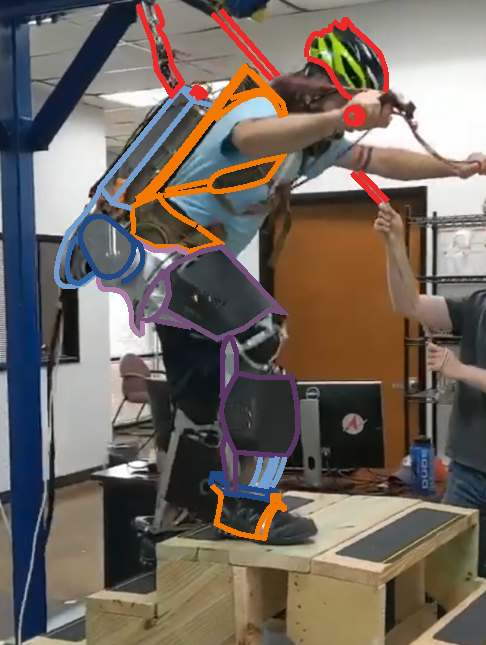
\includegraphics[width=.5\columnwidth]{exo_parts.pdf}%
	\caption{The Apptronik Sagittarius Exoskeleton used in this paper. The operator can climb stairs with the exoskeleton, even when it is not amplifying forces, due to the backdrivable torque-controlled actuators (gravity compensation and strength amplification are both active in the pictured movement). Coloring segregates rigid exoskeleton parts for the right leg (blue-through-purple), human interfaces (orange) and the safety features (red).}\label{fig:parts}
\end{figure}

%% Fig:parts and safety features of the exoskeleton
The different parts of the exoskeleton are highlighted in Fig.~\ref{fig:parts}, with rigid bodies being bordered by different color lines on the spectrum from blue to purple, human attachment points in orange, and safety features in red. To ensure the safety of the operator, the exoskeleton is attached via a slack safety rope to an overhead gantry system, and the rope's height is operated by an assistant when the height is changing rapidly (as in the stair-climbing \ta{activities} pictured in Fig.~\ref{fig:parts}. The operator wears a helmet, and there are multiple easy ways to stop the exoskeleton in an emergency: 1) a software emergency stop button, 2) a button on the top of the main backpack circuitry box, and 3) a button that the operator is required to hold at all times. 


\subsection{Controller Implementation}
While we have presented the controller design in a very general way, not all of its nuanced behavior is relevant enough to demand implementation in the hardware system we used. In particular, the dynamic terms in \eqref{eq:dynamic_equilibrium} were not large enough for the operator to notice their omission, and the dynamically consistent pseudo-inversion of $\mathbf J$ is unnecessary given that $\mathbf J$ is invertible with the tasks we defined, thus
\begin{equation}
\mathbf f = \mathbf J^{-T} (g_e - S\tau).
\end{equation}
Note that when a \ta{component of the \emph{amplification task}} has $K(s)$ set to zero, it \ta{will not amplify human forces but will still compensate gravity.}

% 1->2 reparameterize foot motion error rows by foot_center and foot-spread
% 2->3 adding in monopod motion row and monopod force column
% 3->4 adding in passive torques
% 4->5 new hip and diff error rows replacing monopod motion and foot spread
% 5->6 addition of a two part cost function on difference error

% controller overview
To summarize the tasks of the controller, the six individual \ta{spatial force vector} components \ta{of the human-side force} are fed into a diagonal matrix of amplification compensators as described in Sec.~\ref{sec:fd}. \ta{And this occurs in the frame of the \emph{amplification task}---the hip frame.} For the three sagittal plane forces and torques ($x$-force, $z$-force, and $y$-torque) we may apply non-zero amplification, but the other three are left at zero in this work. This is based on the physical intuition that the sagittal plane forces and torque represent the larger interaction quantities during walking. This forms the 6-DOF \ta{\emph{amplification task}}.
Based on a bed of 12 insole-mounted pressure sensitive resistors, a rough estimate of the human center of pressure is produced. This estimate is used to construct the elements of the \ta{\emph{inter-foot force task}}, which is also a 6-DOF task.
With this hardware-specific pre-processing completed, the tasks are sent to a separate and more generic module to perform the linear programming optimization work. The software implementation of this optimization process is separate from the Apptronik control framework and is available as open source software \cite{Thomas2019LPExo}. It primarily acts as a wrapper layer for the linear programming solver from the COIN-OR \cite{LougeeHeimer2003IBM} community.

%% Paragraph about fig:cartoon
Fig.~\ref{fig:cartoon} describes the sensor configuration on the Sagit exoskeleton and contrasts this to the way we visualize the behavior of the optimization problem. Fig.~\ref{fig:cartoon}.a shows the HCRL logo wearing the exoskeleton, colored dark gray for the structure of the exoskeleton, yellow for the visible force sensors, and green for the parts of the exoskeleton that are considered to be part of the human (the human attachments). In Fig.~\ref{fig:cartoon}.b only the exoskeleton and the sensors are displayed, revealing the shoe inserts, with sensorized pads and an additional force sensor on the back. In Fig.~\ref{fig:cartoon}.c we label the three human attachments as they are numbered in the code. Fig.~\ref{fig:cartoon}.d introduces the visualization of the optimization configuration, where the operator (without its mass) and the exoskeleton are grounded at attachments which happen to correspond to the human interfaces.
With the exoskeleton and massless operator hanging from these grounding points, the job of the exoskeleton is to choose the joint torques that minimize some cost\ta{, and this cost essentially identifies two groundings to avoid using (Fig.~\ref{fig:cartoon}.e).}
For example, if the steady state amplification rate is non-amplifying, i.e. $\alpha_0=1$, then the \ta{\emph{amplification task}} directly penalizes the 1-norm of forces on ground 0---the fictitious connection between the exoskeleton and the world at the backpack. When the human's weight is on the left foot (interface 1) the foot cost penalizes the 1-norm of ground 2---the right foot's friction grounding, resulting in the robot deciding to support its weight as far as possible from ground 1---the left foot. The significance of the massless operator is that the optimization gives an allowance for the human to help the shared-control system exceed the limitations of the robot's own actuators. This means the robot is unlikely to abandon part of a task simply due to the passive joints, but it will if achieving this task would put unreasonably high strain on the human's ankle roll and hip yaw joints.

\begin{figure}[tb]\centering\resizebox{.9\columnwidth}{!}{
	\def\svgwidth{\columnwidth}
	{%\footnotesize%
		\input{exo_cartoon.pdf_tex}%
	}}
	\caption{\ta{
To visualize our optimization problem's behavior, we consider our exoskeleton (a) and the difference between its real force sensor configuration (shown in b) and the three human interfaces the optimizer cares about (shown in c). The optimizer treats the operator as massless and assumes the three interfaces are contact constraints (d). The optimizer is aware of the mapping between the exoskeleton joint torque vector and the reaction forces at the three constraints. With the exoskeleton and massless operator hanging from these grounding points, the job of the optimizer is to choose the joint torques that minimize the cost function\ta{, and this cost essentially identifies two groundings to avoid using (Fig.~\ref{fig:cartoon}.e).} The result is that the cost function guides the exoskeleton to support the system's weight from the stance foot, at least when this does not conflict with the foot contact constraints or joint torque limits. While not explicitly pictured, the \emph{amplification task} simply shifts the ``zero'' point for the cost function's penalty on the e.0 contact (measured by the b.0 force/torque sensor, and felt by the operator through the c.0 backpack attachment).
}}\label{fig:cartoon}
\end{figure}

\subsection{Priorities}

%% Setting priorities
\ra{One might suspect that the order of task importance would be easy to determine a priori, but it was a rather empirical weighting process in practice.}%
\ta{We iterated various priority rankings between the components of the \emph{amplification task} until our operator was satisfied with the behavior.}
\ra{First, seeking to fall back to the linear inverted pendulum behaviors of a point foot robot (that is, prioritizing amplification in the direction between the center of mass and the center of pressure as well as amplification in hip pitch---similar to the hip tasks of the Hume biped \cite{KimEA2016TRO}) we found them to frustrate the operator with their naturally unstable lateral position.}%
\ta{First, we attempted to re-create linear inverted pendulum behavior by prioritizing the moment components over the force components. This prioritization had been effective with the Hume biped robot \cite{KimEA2016TRO}. Unfortunately, this first approach frustrated the operator, as the exoskeleton was naturally unstable.}
\ta{We eventually settled on the weightings in Tab.~\ref{tab:priorities}, which sacrifice $x$-torque first and are more comfortable for the operator.}
\ta{This} preference may be exoskeleton or operator specific.
The main \ta{drawback of the priorities from Tab.~\ref{tab:priorities}} is that at each stance transition the hips of the device roll such that the stance hip is higher than the swing hip---likely due to the lower penalty on hip amplification $x$-torque.
However, we must sacrifice something, and this appeared to be the least-uncomfortable choice. The large swing in the hip position is due to the rather loose coupling that the backpack provides in this degree of freedom.

\begin{table}[tb]\centering
	\caption{Implemented Task Priorities}\label{tab:priorities}
	\begin{tabular}{cc}
		\toprule
		Task & Weighting\\
		\midrule
		Hip Amplification $x$-Force & $1\times 10^{5}$\\
		Hip Amplification $y$-Force & $1\times 10^{5}$\\
		Hip Amplification $z$-Force & $1\times 10^{5}$\\
		Hip Amplification $x$-Torque & $1\times 10^{0}$\\
		Hip Amplification $y$-Torque & $1\times 10^{1}$\\
		Hip Amplification $z$-Torque & $1\times 10^{5}$\\
		\ta{Inter-Foot} $x$-Force, Limit Penalty& $1\times 10^{-1}$, $1\times 10^{5}$\\
		\ta{Inter-Foot} $y$-Force, Limit Penalty & $1\times 10^{-1}$, $1\times 10^{5}$\\
		\ta{Inter-Foot} $z$-Force, Limit Penalty & $1\times 10^{-6}$, $1\times 10^{6}$\\
		\ta{Inter-Foot} $x$-Torque, Limit Penalty & $1\times 10^{-6}$, $1\times 10^{5}$\\
		\ta{Inter-Foot} $y$-Torque, Limit Penalty & $1\times 10^{-6}$, $1\times 10^{5}$\\
		\ta{Inter-Foot} $z$-Torque, Limit Penalty & $1\times 10^{0}$, $1\times 10^{5}$\\
		\bottomrule
	\end{tabular}
\end{table}

%\subsubsection{Limit Penalties for Ground Contact}
In testing, we began to suspect that operators may prefer a lower task penalty on the \ta{\emph{inter-foot force task}} while in double support but react strongly negatively to \ta{\emph{inter-foot force task}} violation while in swing (since this entails the exoskeleton loading their swing foot).
We made a slight modification to the sum scalarized cost for the \ta{inter-foot force task} \ta{as described in \eqref{eq:general_opt}, \eqref{eq:slackplus}, \eqref{eq:slackminus}, and \eqref{eq:e_def}}. \ta{A second copy of the task penalty was added, with a dead zone. We made the \emph{inter-foot force task} error appear \emph{twice} in the task error vector $e(\tau)$ instead of only once as in \eqref{eq:e_def}. Thus, we had two separate components of the weight vector $w$ from \eqref{eq:general_opt} that penalized the same task. To introduce the dead zone for the second copy of the penalty, we added a sparse bias vector to \eqref{eq:slackplus} and \eqref{eq:slackminus}. We call this new penalty, with its dead zone and higher penalty cost, the ``Limit Penalty'' (see Tab.~\ref{tab:priorities}) since it acts like a soft limit forcing the values to stay within the dead zone.} \ta{Within the dead zone, this new cost still behaves like the original weighted 1-norm cost (plus a constant bias that does not influence the optimum), but at the boundary of the dead zone, the weight suddenly becomes much higher.}

We scheduled the dead zone width based on the center of pressure location, such that in single support this dead zone collapsed to zero and the \ta{\emph{inter-foot force task}} essentially took on the higher weighting of the limit penalty. In dual support, the width of the dead zone reached its widest when the feet were evenly balanced and reduced linearly in either direction away from that midpoint. 

%
%% About the limitations of underactuation
%The under-actuation of the exoskeleton (due not to the floating base joint, but to the two passive joints in each leg) prevent this goal from reaching zero, though it would be possible if the exoskeleton were actuated more like a typical humanoid robot. Our exoskeleton cannot walk by itself. It relies on the human to power the passive joints, which leads to an interesting question: should the exoskeleton attempt to meet its goal assuming that the human does not help, or should it anticipate the human's assistance? After all, the human influences the exoskeleton through the contact sensors anyway, so if we penalize the contact sensors, the exoskeleton will always be doing its best to reduce the effort the human needs to apply. This might be the case if we were confident in the quality of our cost function corresponding to the human operator's preference for impeding forces, however this strategy actually led to sudden switching of the desired internal forces for small changes in joint angles. So instead we decided to let the exoskeleton explicitly ignore the cost penalty in the four dimensional subspace corresponding to passive torques by actuating these joints in the optimization and then discarding the result.

%
%$C_1$, $c_1$, $C_2$, and $c_2$ relate to the contact constraints on the exoskeleton's feet. Passive joints on the exoskeleton can be represented in two ways: either they can be removed from the torque vector and $S$, or their torque limits, specific elements of $\bar\tau$, can be set to zero. We adopted the second strategy, but then decided to allow the torque limit to represent not what the exoskeleton can achieve by itself, but what it can achieve with human assistance. In this sense the exoskeleton has no passive joints. Comparisons between treating the passive joints as actually passive, or allowing the exoskeleton to ``trust the human'' suggested that this second strategy seemed to produce more desirable behavior from the operator's point of view, and we ultimately increased the torque limits of all the joints to account for this expected human contribution. A secondary saturation step remained to enforce the actual torque limits of the robot's actuators.


%\begin{subequations}
%	\begin{align}
%	&\underset{\tau}{\mathrm{minimize}}
%	&& \sum_{i=1}^6 (|f_{0,i}(\tau)-\hat f_{0,i}| 10^{w_{0,i}}+|f_{d,i}(\tau)| 10^{w_{d,i}} )\label{exo:eq:1np:cost}\\
%	&\text{subject to}
%	&&|\tau| \leq \bar{\tau},\\
%	&&& C_1 f_1(\tau)+c_1 \geq 0,\\
%	&&& C_2 f_2(\tau)+c_2 \geq 0,\\
%	&\text{where}
%	&&\begin{pmatrix} f_0(\tau)\\f_1(\tau)\\f_2(\tau)\end{pmatrix} = J_r^{-T}(g_e - S\tau) ,\\
%	&&& \begin{pmatrix}
%	f_s(\tau)\\f_d(\tau)
%	\end{pmatrix} = \mathbf G^{-1} \begin{pmatrix} f_1(\tau)\\f_2(\tau)\end{pmatrix}.
%	\end{align}
%\end{subequations}



\begin{figure}[btp]
	\begin{minipage}{2in}\centering\begin{center}\captionof{table}{Experimental Parameters}\label{tab:expparam}\end{center}\vspace{-.25in}
		\begin{tabular}{cccc}
			\toprule
			Test & SBC\ta{$^\dagger$} & $\alpha_0$ & Load\\
			\midrule
			\ref{subs:amp}.1 & Off & 0 & 0 N\\
			\ref{subs:amp}.2 & On & 0 & 0 N\\
			\ref{subs:amp}.3 & On & 0 & 110 N\\
			\ref{subs:amp}.4 & On & 3 & 110 N\\
			\bottomrule
		\end{tabular}
		\vspace{.5em}
		
		\ta{\scriptsize$\dagger$---Shared-Body Controller (SBC) enabled.}
		
		\captionof{figure}{Load position in \ref{subs:amp}.3 and \ref{subs:amp}.4. Load hangs from a chain attached to the exoskeleton. Human effort measured with a six-axis force torque sensor, highlighted in red. Measurements are presented in the pictured ``hip center'' coordinate frame.}\label{fig:experimental_condition}
	\end{minipage}
	\begin{minipage}{1.3in}
		\centering\resizebox{1.2in}{!}{
		\def\svgwidth{1.3in}
		\input{experimental_condition.pdf_tex}}
	\end{minipage}
\end{figure}

\begin{figure*}[tb]%
	\centering\resizebox{1\textwidth}{!}{\def\svgwidth{\textwidth}\footnotesize%
	\input{experiment_v2.pdf_tex}}%
	\caption{\ta{The four experiments from Tab.~\ref{tab:expparam}, shown as subfigure columns A--D, are compared in terms of the three sagittal plane components of the human--robot interaction force/torque, the sagittal joint torques, and the sagittal joint angles. In Exp.~\ref{subs:amp}.1 (A), the exoskeleton joints apply no torque (as shown in A.4), and the human--robot interface supports $\approx300$ N (as shown in A.3) as well as a $\approx35$ Nm moment at the hip (as shown in A.1). In Exp.~\ref{subs:amp}.2 (B), the controller is turned on with $\alpha_0=1$ (no amplification), and human--robot vertical force (B.3) and sagittal torque (B.1) are vastly decreased due to gravity compensation. In Exp.~\ref{subs:amp}.3 (C), a 11~kg mass is attached to the back of the exoskeleton (as shown in Fig.~\ref{fig:experimental_condition}), and this produces an increase in the human--robot sagittal torque (C.1), $\approx30$ Nm. Finally, Exp.~\ref{subs:amp}.4 (D) increases $\alpha_0$ from 1 (no amplification) to 3 in the sagittal tasks, and the human--robot sagittal torque increase due to the added mass is reduced by roughly a third---considering B.1, C.1, and D.1 representing the average numerical value of the curves, D.1 $-$ B.1 $\approx 1/3($C.1 $-$ B.1$)$---as expected. With the amplification engaged, the operator deepens the squat at 10 seconds (D.5) and then moves to a second, less extreme squat at 20 seconds (D.5), showing that the torque reduction continues to work. This squat is shown in the video attachment  \cite{Thomas2020Youtube}. We would also expect that amplification would reduce the vertical force from the added mass; however, the vertical force remains roughly zero before adding the weight (B.3), after adding the weight (C.3), and with both the weight and amplification (D.3)---the expected 110 N force increase between (B.3) and (C.3) did not occur. Since the operator recalls feeling vertical forces from the addition of the mass, we suspect that there is a ``force leak'' where the vertical component transferred to the operator in a way the force sensor could not detect. Torque and angle measurements in the bottom two subfigure rows are measured using the robot's spring deflection encoders and joint encoders, and therefore represent the robot's---and not the operator's---torque and position.}
	}\label{fig:experiment}
\end{figure*}

\subsection{Demonstrating the Amplification Task}\label{subs:amp}
We conducted a set of simple tests to demonstrate the difference between gravity compensation and human strength amplification. These tests aimed to demonstrate an improvement in amplification stability relative to previous controllers developed for the exoskeleton and its previous partial prototypes (the 1-DOF testbed from \cite{HeThomasPaineSentis2019ACC,ThomasCoholichSentis2019AIM}, a two degree of freedom leg, and a previous revision on the same lower-body design) under the same project \cite{Campbell2018Thesis}, which was a condition of our using the exoskeleton.\footnote{Which is to say, our testing time was limited, and the scope of our experiments was narrow.} 

Fig.~\ref{fig:experimental_condition} and Tab.~\ref{tab:expparam} show the basic structure of our tests: the operator wears the exoskeleton in a roughly standing position and various controller features are turned on and off. Extra weight is attached to the backpack as an unknown load in tests \ref{subs:amp}.3-4, and the image shows where it hangs relative to the operator. Fig.~\ref{fig:experiment} shows the results of the three tests. 

 
\subsection{Discussion of The Amplification Task}\label{subs:amp_disc}

In the first test, \ref{subs:amp}.1 the exoskeleton joints are on, but the desired torque is zero. The first column of plots in Fig.~\ref{fig:experiment} show the large $z$-force on the backpack due to the gravitational load of the exoskeleton acting on the operator. Variation in the angle shows that the operator was not perfectly holding still over the duration of the test. This, while it prevents us from easily comparing across experiments (the operator does not even have the same resting posture between loading configurations) is hard to compensate for or avoid.

The next test, \ref{subs:amp}.2 enables gravity compensation---which means the torques from the shared-body controller are applied to the robot, but the amplification filters are all set to apply no strength amplification feedback ($\alpha_0=1$, so $f_a^d=0$). This drastically reduces, but does not entirely eliminate, the interface forces and torques. Even if the robot's mass parameters were perfectly modeled, the operator would still need to apply forces through this interface to control the passive joints of the robot. Compensating for the weight of the heavy exoskeleton is the most significant component of the system's behavior\ta{. We can see this from the enormous reduction in human interface forces and torques in Fig.~\ref{fig:experiment} between \ref{subs:amp}.1 and \ref{subs:amp}.2: the vertical force, Fz, drops roughly 300 Newtons, and the sagittal plane torque, Ty, drops roughly 40 Newton meters.}

In test \ref{subs:amp}.3, we added an 11 Kg (25 lb) mass to the backpack, without changing the control mode. \ta{Based on our empirical determination, this represents the maximum load the exoskeleton could reliably handle without overheating during dynamic motions like walking.} The test does not focus on the transient response but on the steady state behavior with the weight (mechanically, it would be hard to make the weight addition appear sudden without dropping it).

We see some unexpected behavior in the vertical sensor force: the weight's 110 N \ta{did not transfer to the sensorized interface}. \ta{The user confirmed that additional vertical force and sagittal torque were felt.} This suggests a ``force leak'' in the design of the backpack sensor, where the force of the added weight is transferred to the operator without passing through the sensor. A likely culprit is the hip-pad of the backpack (directly connected to the operator) and the hips of the exoskeleton---as this would be consistent with the clear increase in the $y$-torque. \ta{The ``force leak'' does not appear to allow all vertical forces to bypass the sensor. \ref{subs:amp}.1 clearly shows large forces.}

\begin{figure*}[t]%
	\centering\footnotesize
	\resizebox{.9\textwidth}{!}{\input{frames_of_demo_compressed.pdf_tex}}
	\caption{Frames from the demo. Frames a.1-5: climbing stairs with amplification but no added weight. Frames b.1-5: walking around. Frames c.1-3: walking around with amplification and extra weight.}\label{fig:demo}
\end{figure*}

In the final test, \ref{subs:amp}.4, we engaged the amplification filters---providing a steady state amplification factor of 3, and a zero pair at 1 Hz for all three degrees of freedom in the sagittal plane.
By choosing these conservative settings, we were able to achieve stability on the first try.\footnote{A later gain-tuning experiment revealed that the bandwidth limit is higher than this, but we ran out of time for exhaustive identification of this limit.}

\ta{
Our system is pioneering in that it amplifies human strength at the backpack/hip link of the exoskeleton; there are no direct performance comparisons for this control feature.
Our steady state amplification of human forces by 300\% exceeded the 208\% amplification (52\% mass reduction) of sagittal hip moment in \cite{ZanottoAkiyamaStegallAgrawal2015TRO}, which also used force feedback to amplify human lower-body strength.
However, this is not an exact comparison, as \cite{ZanottoAkiyamaStegallAgrawal2015TRO}'s system used a treadmill mounted exoskeleton, had a different sensing configuration, and has only two degrees of freedom whereas our system has 12.
The amplification's pole frequency (.58 Hz) and amplification magnitude ($\alpha_0=3$) at the hip/backpack human--robot interface are comparable to our previous results on a 1-DOF human elbow exoskeleton; in the notation of Appendix A, \cite{HeThomasPaineSentis2019ACC}'s robust controller used $\alpha_0=10,\ k_G=0.1,\ Z_g=10,\ \text{and}\ P_g=0.01,$ resulting in an amplification magnitude of 2.995 at 0.58 Hz.
However, unlike our controller, \cite{HeThomasPaineSentis2019ACC} had even greater amplification at lower frequencies: its lowest pole-pair was at $0.146$ Hz, and its steady state amplification rate was 9.91.
%In terms of \emph{mechanical} performance, our preliminary testing suggests a payload capacity of $\sim$11-23 kg, which is lower than \cite{Kazerooni2005IROS}'s 34 kg.
}

As shown in Fig.~\ref{fig:experiment}'s fourth column, the human's effort was reduced to roughly a third of its value in the third column in the $y$-torque component.
\ta{More specifically, the disturbance due to the added weight, which can be seen by comparing \ref{subs:amp}.3 (with weight) against \ref{subs:amp}.2 (no weight) in terms of y-axis torque, is attenuated by the amplification factor, resulting in a much smaller disturbance effect when comparing \ref{subs:amp}.4 (attenuated weight) to \ref{subs:amp}.2 (no weight). We must make this comparison despite joint angle differences on the order of 10 degrees between these tests---a limitation of our operator and operator--robot coupling. In \ref{subs:amp}.4, the operator engages in two different squat positions (switching posture at roughly 10 and 20 seconds). The interface forces remain within 10-15 Nm despite these kinematic changes. This supports the notion that if the operator were able to perfectly reproduce the posture from Exp.~\ref{subs:amp}.3 in \ref{subs:amp}.4, the y-axis torque would also be within this range.}


\subsection{Discussion of Foot Transitions}




 \begin{figure*}[htbp]%
 	\centering%
	\resizebox{.85\textwidth}{!}{\input{transitions_small.pdf_tex}}\vspace{-.15in}
 	\footnotesize%
% 	\begin{tabular}[t]{cc}%
% 	\begin{minipage}[t]{.5\textwidth}%
 	\begin{tabular}[t]{rl}%
 		\toprule
 		Callout & Description\\
 		\midrule
 		a.0 & The base or hip frame\\
 		a.1 & The frame of the backpack's  force/torque sensor\\
 		a.2 & Visualization of child frame  to parent frame vectors\\
 		a.3 & (Obscured) frame of the left hip adductor joint\\
 		a.9 & (Clearly visible) frame of the right hip adductor joint\\
 		a.4/a.a & Frame of the left/right hip flexor joint\\
 		a.5/a.b & Frame of the left/right passive hip ``yaw'' joint\\
 		a.6/a.c & Frame of the left/right knee flexion joint \\
 		a.7/a.d & \begin{minipage}{2.75in} Frames of the left/right ankle flexion and passive ankle roll joints (hard to distinguish) \end{minipage}\vspace{.025in}\\\vspace{.025in}
 		a.8/a.e & \begin{minipage}{2.75in}Frame of representation for the constructed sum/difference reaction force vectors---momentarily coincident with the (not visualized) left/right foot bottom frame due to single support\end{minipage}\\
 		b.0 & Spatial force vector (SFV) of the backpack force/torque sensor\\
 		b.1 & \begin{minipage}{2.75in}SFVs of the left and right foot structural force/torque sensors, expressed in the ankle frame\end{minipage}\\
 		\bottomrule
 	\end{tabular}%
% \end{minipage}%
%&%
%\begin{minipage}[t]{.5\textwidth}%
	\begin{tabular}[t]{rl}
 	\toprule
 	Callout & Description\\
 	\midrule
 	b.2 & Optimal reaction SFV for the right foot\\
 		b.3 & Frame of the representation for the \ta{inter-foot} SFV\\
 		b.4 & Robot contribution to optimal sum SFV \\
 		b.5 & Measured sum SFV (from structural sensors)\\
 		b.6 & Optimal sum SFV\\
 		c.0 & Measured backpack SFV in hip frame\\
 		c.1 & Robot gravity SFV visualization \\
 		c.2 & Robot gravity compensation SFV visualization\\
 		c.3 & Measured human COP (ankle origin weighted average) \\
 		c.4 & Frame of rep. for sum SFV \\
 		c.5 & Frame of rep. for \ta{inter-foot} SFV\\
 		d.0 & Optimal robot joint torques \\
 		d.1 & Applied robot joint torques (filtered and saturated) \\
 		d.2 & \begin{minipage}{2.75in}Individual FSR relative magnitude visualization for the 12 sensors of each foot, used to estimate within-foot center of pressure\end{minipage} \\
 		\bottomrule
 	\end{tabular}%
 %\end{minipage}\end{tabular}
 	
 	\caption{Human weight transfer in 0.2 seconds (subfigures evenly spaced in time) showing the exoskeleton visualization in the rviz program.}\label{fig:transitions}
 \end{figure*}
 
 
\ra{With or without amplification, the primary behavior of the system was to use shared-body control to partially compensate the robot's own gravity while allowing human-led foot transitions through the \ta{\emph{inter-foot force task}}.}\ta{Distributing weight between the two feet using the \ta{\emph{inter-foot force task}} is a key behavior of the system and was tested when the operator walked on level ground and stairs.}
Since the robot itself was based on high bandwidth torque-controlled actuation, the operator could easily backdrive it to climb up stairs or to stand on one foot.%
\ra{Since this was the case\ta{,} gravity compensation was the dominant effect of the controller, with amplification acting in a supplemental role.
But \ta{with or without amplification}, the control of the contact transitions via the \ta{\emph{inter-foot force task}} was key.}
\ta{While this happened, the exoskeleton continued to compensate for its own gravitational weight and amplify strength at the hip/backpack sensor.}


%The amplification was certainly the less obvious of the behaviors, yet was still perceived as beneficial.
 %Since there was no reason to manipulate the environment with the exoskeleton's backpack---it essentially just compensated for the error in the gravity compensation term.
 
\ta{Fig.~\ref{fig:demo}.b and Fig.~\ref{fig:transitions} show the operator shifting weight from one foot to another and lifting up the legs one at a time.}
\ta{This behavior highlights the human-led foot contact transitions and demonstrates how the weight is shifting in \emph{anticipation} of the actual contact transition.}
\ta{As mentioned in Sec.~\ref{sec:ift}, the weighting matrices $Q_1$ and $Q_2$ in \eqref{eq:Q1Q2def} are scheduled according to the robot's measurement of the human's weight distribution.}
When the human shifts weight to one foot, the $Q$ matrix penalty for reaction forces on the other foot becomes much larger. And since this causes the COP of the robot to approximate the COP of the human, this prevents the human from needing to lift a load-bearing robot leg. In addition, the penalty limit method allowed the exoskeleton more freedom during dual support but smoothly reduced this freedom when approaching single support, so that by the time it was reached the \ta{\emph{inter-foot force task}} was essentially the highest priority.
 
 This behavior is shown in more detail through the internal robot visualization of Fig.~\ref{fig:transitions}.
 This Rviz model manages to show almost everything that is going on, as described in the legend table.
 All frames are expressed as red ($x$) green ($y$) blue ($z$) line segments meeting at the local origin.
 Spatial force vectors (comprising a force and a torque) are shown as a ray from the local origin (the force) and a bi-vector---a directed plane comprised of four vectors making a square---to represent the torque. Joint torques are represented as pure bi-vectors.
 Unlike vector descriptions of torque, the bi-vector visualization has an unambiguous scaling relative to the force visualizations and cannot be confused for them.
 The four instants pictured in Fig.~\ref{fig:transitions} of the contact transition show the apparent center of pressure moving from the left foot to the right foot, and the corresponding shift in all the joint torques and the predicted reaction forces from the shared-body controller.
 As this is shifting, the reference frame of expression for the sum of reaction forces and the \ta{\emph{inter-foot force task}}'s difference of reaction forces swap feet.
 At all times, the reaction force/torque b.6 representing the sum is roughly equal to the sum ground reaction force calculated without using the passive joints b.4---which means that the robot is supporting the vast majority of its weight even during this transition.
 The backpack force/torque sensor b.0 confirms this, as it is small (and therefore hard to spot) throughout the transition.


% Table of footstep transition parameters?










%%%%%%%%%%%%%%%%%%%%%%%%%%%%%%%%%%%%%%%%
%%%%%%%%%%%%%%%%%%%%%%%%%%%%%%%%%%%%%%%%
%%%%%%%%%%%%%%%%%%%%%%%%%%%%%%%%%%%%%%%%
%%%%%%%%%%%%%%%%%%%%%%%%%%%%%%%%%%%%%%%%
%%%%%%%%%%%%%%%%%%%%%%%%%%%%%%%%%%%%%%%%
\section{Discussion}\label{sec:disc}

% return to high level
\ta{
Strength amplification control offers us the potential to feel stronger as we manipulate the environment (including the loads) through our exoskeleton.
This paper provides a framework that has put that vision into practice under laboratory circumstances, albeit with an exoskeleton that was not originally designed to manipulate the environment.
}


\subsection{\ta{Benefits and Drawbacks}}
% What can it do (potential benefits) What kind of control performances are newly achieved How does this improve over the state of the art
\ta{
This framework has several advantages relative to the state of the art.
It respects contact limitations---guaranteeing that the exoskeleton will never force the person to roll their ankles, lift their toes, or slide their feet.
It improves human-side compliance relative to the gravity compensation baseline without the anti-stable acceleration feedback of \cite{KazerooniRacineHuangSteger2005ICRA}.
It keeps the human in control of the inter-foot force distribution using an elegant linear algebraic decomposition of the contact forces---a more general approach than Ref.~ \cite{JacobsenOlivier2014Patent}.
It allows the operator to move heavy objects without removing the force-feedback path that they would need in order to move the objects carefully---a force-feedback path that is removed by admittance control strategies \cite{FontanaVertechyMarcheschiSalsedoBergamasco2014RAM}.
}

% What can it not do (potential drawbacks)
\ta{
Of course, the framework has downsides as well.
The strategy depends on centralizing the contact between the human and the exoskeleton into a small set of sensors.\footnote{\ta{With one foot on the ground, our exoskeleton measures the human at two places: the hip/backpack attachment and the swing foot attachment.}}
This centralization places a significant burden on the mechanical design and introduces a new failure mode---the ``force leak,'' where interaction between the robot and the operator occurs outside the sensors.
Additionally, all amplified interaction with the environment must go through the exoskeleton structure---another mechanical design challenge.
Due to the complexity of the mechanical design problem, the strategy makes it difficult to achieve the ultra-high energy density of successful locomotion augmentation exoskeletons \cite{KimWalshEA2019Science,MooneyRouseHerr2014JNRE}.
This is an open problem.
Augmentation exoskeletons are already close to the energy-density boundary at which the energy they provide is equal to the energy they cost the user due to their mass.
The extra design constraints make it harder for amplification exoskeletons to cross this boundary even at slow walking speeds.
}


\subsection{\ta{Open Problems in the Control Framework}}
\label{subs:open_control}
% open questions in the control framework: 1: human approximation
\ta{The control framework itself also has some open questions.
First, we approximated the mechanical impedance of the human and the cuff as being component-wise decoupled between the six degrees of freedom in our \emph{amplification task}.
Since an extremely low amplification bandwidth is still stable, and since our tuning process increases bandwidth until instability is discovered, this approximation limits us by introducing conservatism in the final tuning. %
Because of inter-component human coupling behavior, the tuning process may result in a different answer depending on the order with which the individual task sub-component bandwidths are tuned. %
}


% second: scalability Address generality and scalability
\ta{Second, the framework was only tested with six \emph{amplification task} sub-components.
In theory, it supports arbitrarily many task sub-components.
And it is also theoretically possible to join the \emph{inter-foot force task} with the \emph{amplification task}---to make the swing foot capable of acting like an amplified manipulator.
We lacked the sensing configuration for such a test: it would require the full 6-DOF interaction force/torque between the human foot and the exoskeleton foot to be measured, rather than just the vertical pressure between them.
Thus, to validate the scalability our theory predicts, we would need an exoskeleton with either A) more sensorized human contacts (arms, for example) or B) the elimination of all human--environment contact that does not pass through the exoskeleton as an intermediary.
}


% 3rd: automoatic Controller tuning: is it task-dependent? Can controller tuning be automated?
\ta{Third, the controller tuning process is intended to be robust to all activities the operator performs, but we cannot know all these activities beforehand.
A practical extension to this work would be to introduce an always-online learning process to continually adapt the tuning and avoid instability.
Previously we have looked at tuning automation using online stiffness estimation \cite{HuangCappelThomasHeSentis2020ACC}.
However, this type of automation could potentially be simpler: if the system starts to vibrate, it could reduce the amplification bandwidth until the vibration subsides.
This is essentially how we tuned the system manually.}

% automatic tuning, but higher performance.
\ta{On the other hand, higher performance might be obtained with a more complex strategy: modeling the human and redesigning the controller.
Modeling the human online could draw on convex programs that automatically learn bounded-uncertainty models \cite{ThomasSentis2019TAC}. 
With this more versatile system identification approach, even a human stiffness with `off-diagonal' terms could be learned.
With every change to the model of the human stiffness bounds, robust control theory could synthesize a transfer matrix $\mathbf K(s)$ that guarantees stability.
}

% address Rmk.~\ref{rev7:proper_discussion}.F: no ground contact
\ta{Finally, the approach makes an assumption that a foot is always on the ground---and this precludes interesting applications in free-fall, underwater (with neutral buoyancy), or micro-gravity.
In such circumstances, the \emph{amplification task} and \emph{inter-foot force task} structures would need to be combined together and significantly altered.
A ``virtual single foot contact'' would not exist.
In its place, the \emph{change in centroidal momentum} \cite{KoolenEA2016IJHR} would need to become the component of torque-space left intentionally unconstrained by the tasks.
The remaining DOFs in torque-space would then be the subject of the new combined amplification task.
The assignment of intuitive and easy-to-tune amplification controllers to such a task---which would concern an ever-changing subspace of the end-effector contact force space---is an open problem.
However, the approach to parameterizing the \emph{internal forces of multi-contact} from \cite{SentisParkKhatib2010TRO} would be a reasonable starting point.
}

\subsection{\ta{Series Elastic Actuators}}

%Benefits and drawbacks of the compliant actuators
\ta{Our exoskeleton hardware features series elastic actuators that are force/torque-controlled, and this decision also comes with benefits and drawbacks.
To our knowledge, this paper is the first demonstration of Multi-DOF amplification control based on human interface force sensors and actuator force sensors (i.e. the series elastic elements).
While such actuators are commonly used in wearable robots, they are a key part of our strategy, because with them we can avoid sensorizing the external force interface.
This is a major advantage compared to systems designed to follow the extender concept \cite{KazerooniGuo1993JDSMC}.
The lack of environment sensors gives us the freedom to properly handle amplification for environmental contract forces at any contact point along the structure of the exoskeleton (or at least in double support---we would need to amplify the \emph{inter-foot force task} to amplify contact between the environment and the swing leg).}

\ta{As for series compliance itself, however, control performance would be slightly better off with nearly-rigid springs.
The series elastic actuators are simply torque sources to us, and direct drive motors offer higher bandwidth as torque sources.
Removing the springs could also save weight.
But series elasticity has some practical advantages: the force sensing is cheap and high quality, the robot's motors are protected from impacts, and both the transmission's friction and the rotor's reflected inertia are well hidden from the user.
}

\subsection{\ta{Potential Applications}}

% Clear purpose, not ``non-repetitive and unpredictable''
\ta{
We have demonstrated the control framework on the Apptronik Sagittarius exoskeleton, which is designed to lift heavy body-distributed payloads as the user moves quickly.
In this use case, the benefit of amplification control---relative to gravity compensation of the payload---is the potential reduction of inertial forces the user needs to compensate (without resorting to acceleration feedback) and the forces due to modeling error in the compensation.
But this is not necessarily the most impactful application area for amplification as a technology.}

\ta{To really see the potential of amplification, we would need to imagine an exoskeleton that was built for heavy-duty environmental manipulation.
Such a system would need to move very slowly but with very high forces.
If it were to move fast, it would require significantly more impressive power density than we typically see today.
Such an exoskeleton, worn by a skilled operator, might be fielded in difficult terrain as an alternative to tracked construction vehicles, with specialized tools for manipulating the environment.
These tools might be so massive that there exists no viable alternative for using them in unstructured environments.
The exoskeleton would act as an adjustable bracing system that allows the operator to maneuver them into position.
Perhaps the operator is a sculptor who uses the exoskeleton to lug a massive jackhammer up the mountainside in order to carve an ornamented staircase for tourists.
Or maybe a forestry service worker is using it to operate a chainsaw at the end of a 24-foot telescoping pole.
%% TODO: be very inventive here.
Exoskeletons as platforms opens up the door to new industrial tools and potential job sites---all because they combine the maneuverability of people with the strength of machines.}

% What problem is our control framework equipped to solve---out there industrial non-anthropomorphic tool holder.
\ta{Our exoskeleton is designed to mimic the kinematics of the person wearing it, but this is not the only way to go about the design. The control framework also has the potential to allow non-anthropomorphic legged robots to amplify human interaction. Imagine, for example, a robot connected to an operator's feet with long spindly legs that join together at a robot 'hip'. This hip also features an enormous power tool that requires the user to manipulate it with both hands. This architecture would require the same control system features as our anthropomorphic exoskeleton structure: strength amplification in the frame of the robot's hip, awareness of contact inequalities, and human-led footstep transitions.}

	

\ra{
%% Limitation: stabilized by human
Due to the inevitable phase loss in the amplification, we remark that the stability of amplification depends on the damping properties in our model of the human. If we were to replace the operator with a series-elastic mechanical dummy of comparable joint stiffness, we would need to change our human-side compliance strategy to remain stable---introducing damping-like behavior near the point of magnitude crossover. Fortunately, humans appear to be quite cooperative with these aggressive controller designs, as has been noted earlier for controllers based on acceleration feedback \cite{Kazerooni2005IROS}---another strategy which increases the human-side compliance of the device.}

% Goes into other sensor configurations (warning: not necessary)
% re-cast as extenability beyond centralized human interfaces?
\ra{Exoskeletons can be designed for multiple sensor configurations, and in this paper we considered exclusively the configuration where the human--robot interface is sensed. This is hardly the dominant paradigm in exoskeleton mechanical design, as it tends to require a massive exoskeleton. However, amplification shaping could also be achieved with only environment--exoskeleton sensors, as such exoskeletons are also able to distinguish, and therefore control, the human-side and environment-side compliance. This could particularly benefit exoskeletons designed to augment the strength of the elderly and volitional stroke patients, which typically use this sensor configuration to reduce the hardware weight.}


\appendices
\section{Relation to Earlier Controller Design Framework}

\ra{In our own prior work in exoskeleton control, we}\ta{The control strategy we previously published in \cite{HeThomasPaineSentis2019ACC} can also be re-expressed in terms of an amplification transfer function. Ref.~\cite{HeThomasPaineSentis2019ACC}} explored the creation of amplification controllers based on reduction of an ``ideal amplification error signal'' $Y(s)=(\alpha_0-1)F_H(s)-\eta(s) F_A(s)$ (in the notation of Sec.~\ref{sec:fd}) using a feedback compensator $G(s)$, with desired actuator force $F_A(s) = G(s) Y(s)$. This left us with a feedback stability model that required system identification of the human. Our proposed structure for $G(s)$ was that of a first order lag filter. The purpose of this section is to explain this prior approach in terms of the modified human-side compliance.

We can eliminate the self-referential $F_A(s)$ definition using algebra:
\begin{gather}
F_A(s) = G(s)((\alpha_0-1)F_H(s)-\eta(s) F_A(s)),\\
%(1+G(s)\eta(s))F_A(s) = G(s)(\alpha_0-1)F_H(s)\\
F_A(s) = \frac{G(s)(\alpha_0-1)}{(1+G(s)\eta(s))} F_H(s).\end{gather}
We also have a first order lag model of $G(s)$,
\begin{gather}
%K(s) = \frac{G(s)}{(1+G(s)\eta(s))}(\alpha_0-1)\\
G(s) = \frac{s+z_G}{s+p_G}k_G,
\end{gather}
where $k_G$ is the gain, $z_G$ is the zero frequency, and $p_G$ is the pole frequency for the lag. We can therefore express the equivalent $K(s)$ this strategy is implementing,
\begin{gather}
K(s) = \frac{s+z_G}{s/k_G + p_G/k_G+(s+z_G)\eta(s)}(\alpha_0-1).
\end{gather}
From here, we can see that the strategy results in something close to another lag filter (if we neglect the actuator dynamics to treat $\eta(s)\approxeq 1$). However, in this case the nominal amplification of the strategy is 
\begin{gather}
%\alpha(s) = \frac{\alpha_0 s+\alpha_0 z_G - s - z_G +s/k_G + p_G/k_G + s+z_G}{s/k_G + p_G/k_G+(s+z_G)}\\
\alpha(s) = \frac{(\alpha_0 + 1/k_G) s + (\alpha_0 z_G + p_G/k_G)}{(1+1/k_G)s + (z_G+ p_G/k_G)},
\end{gather}
which is similar to the controller parameterization in this paper, but less convenient because its steady state behavior is not $\alpha_0$ as we might expect but rather $\frac{\alpha_0 + p_G/(k_G z_G)}{1+p_G/(k_G z_G)}$, which will always be less than \ta{or equal to} $\alpha_0$. Nor does it return to the natural system behavior at high frequencies, since the nominal value of high frequency $\alpha(s)$ does not return to unity. (In practice it will still return to unity due to $\eta(s)$).



